\documentclass[a4paper, 12pt]{article}

\author{Peter R.T. Munro}

\title{Documentation for Isotropic Finite Difference Time Domain Code}


\usepackage{graphicx}
\usepackage{verbatim}
\newcommand{\eq}[1]{Eq.\ (\ref{#1})}
\newcommand{\rfig}[1]{Fig.\ (\ref{#1})}
\newcommand{\sect}[1]{Sec.\ (\ref{#1})}
\newcommand{\eqs}[2]{Eqs.\ (\ref{#1}) and (\ref{#2})}
\newcommand{\eqr}[2]{Eqs.\ (\ref{#1}) to (\ref{#2})}
\newcommand{\tab}[1]{Table\ \ref{#1}}
\newcommand{\refs}{Refs.\ }
%\usepackage[dvips]{graphicx} \usepackage{amsmath}
\usepackage{amsfonts}
\usepackage{amsbsy}
\usepackage{amsmath}
%\usepackage{showkeys}
%\twocolumn



% ignore these for the time being, they're margins.
\setlength{\parindent}{0pt} \setlength{\parskip}{1.6ex}

\begin{document}
	\bibliographystyle{unsrt}
	% this starts your document.
	% this includes the title
	\maketitle\tableofcontents
	%\tableofcontents
	\section{Summary}
	This implementation of the Finite Difference Time Domain (FDTD) method is designed to model the scattering by isotropic materials
	including perfect dielectrics, lossy dielectrics and dispersive
	media. Reasonably general incident fields can be modelled, including
	plane waves and tightly focused fields\footnote{Practical restrictions
		are addresed in a later section}. The time dependence of the
	simulation can be either ``pulsed'' or ``steady state''. The FDTD grid must be a cuboid
	and all objects within it are modelled using a stair cased
	approximation. The sides of the Yee cell need not be of equal length
	however each Yee cell in the grid must be of identical
	dimensions. Multilayer structures with a profile uniform along one or
	two dimensions may be modelled. An understanding of much of the
	following will be enhanced by consulting the book by Taflove and
	Hagness \cite{taflove00book}.

	\section{Introduction \& Overview}
	\subsection{Incident field}
	To be strictly correct the incident field should be introduced from
	the sides of a cuboid which surrounds the scattering regions. This is
	known as the ``Total-Field/Scattered-Field'' formulation. This
	implementation allows only for a steady-state simulation using this
	method. This involves slowly ``ramping up'' the inicident field and
	then waiting until the scattered-field reaches a steady state.

	Tightly focused fields may be introduced by using a technique which is
	only strictly correct for waveguides. As long as ``the majority'' of
	the power in the incident field is contained within a single plane of
	the aforementioned cuboid, we can introduce the field from that plane
	only. This allows the use of the so-called pulsed mode where the
	incident field is introduced as a Gaussian modulated pulse. A time
	harmonic solution may be obtained by performing a discrete Fourier
	transform at the frequency of interest, normally the centre frequency
	of the Gaussian spectrum.

	\subsection{Materials}
	Materials comprising both the homogeneous background or multi-layer
	structure as well as the scattering cells may be specified using
	both the means of conductivity and relative permitivity or a
	dispersive model (Drude) may be used.

	\subsection{PML}
	A perfectly matched layer (PML) is implemented so that open scattering
	problems can be modelled. The PML correctly handles the case of
	dispersive and lossy materials as per Gedney
	\cite{gedney96electromagnetics399,gedney96ieeetransantprop1630}.

	\subsection{Field extraction}
	The time harmonic field can be obtained either at each point within
	the FDTD grid or on the surface of a cuboid. The latter is useful as
	it reduces the copmutational and storage requirements whilst allowing
	the field outside the cuboid to be calculated using the Stratton-Chu
	integral \cite{poggio73book,stratton39pr99}. One however must ensure
	that all material inhomogeneities are contained within the cuboid and
	that only the scattered field is used in the Stratton-Chu calculation.


	\subsection{Performing a simulation}
	The software runs in a number of modes. It can be called directly from
	the Matlab command line or be called as a stand alone executable
	taking \verb+.mat+ files as input. Much of the internal details are
	hidden from the user and all inputs are specified from a text-based
	input file. The scattering cells are described using either a
	\verb+.mat+ file or a text file. The typical sequence for performing a
	simulation is as follows:
	\begin{enumerate}
		\item Specify simulation parameters for non-scattering cells in text
		input file.
		\item Construct the scattering cell file.
		\item Use the supplied m-file to either construct the program input
		file or to execute the simulation.\label{it:infile}
		\item In the case that an input file is constructed in step
		\ref{it:infile}, the simulation is executed.
	\end{enumerate}
	\section{Master input file specification}
	%%%
	\subsection{Introduction}
	The finite difference time domain (FDTD) method models the interaction of an incident electromagnetic
	field with a finite volume of space (denoted the computational space)
	composed of dielectric and conducting materials. The computational
	space is divided into cells each of which are identical in size. The
	material properties of each cell may differ however. Scattering
	objects may then be defined by varying the material composition of
	cells to model as closely as possible the geometry of the object to be modelled.

	Many parameters must be set in order to specify a problem to be
	modelled. These parameters can be partitioned into a number of
	categories. For example, the grid size and material composition must
	be specified. The properties of the source must also be
	specified. There are also a number of FDTD specific parameters that must
	also be set. The complete list of input parameter types is given
	below:
	\begin{itemize}
		\item Grid: These control the resolution and size of the
		grid as well as the default material in which scattering objects are
		embedded. Parameters to set the multilayer structure are included in
		this category.
		\item Source: These determine the properties of the incident
		electromagnetic field.
		\item Simulation type: Determines what kind of simulation is
		performed. Allows, for example, a simulation type amenable to
		analysis of the field in the time domain or the frequency domain to
		be chosen.
		\item FDTD specific: Parameters which are specific to the FDTD
		algorithm. These must be chosen by someone with some experience with
		FDTD. Some of the source parameters also fit into this category.
		\item Output: Determines which field parameters are calculated and
		outputed by the algorithm.
		\item Perfectly Matched Layer (PML): This is used to model unbounded
		free space scattering with a finite grid. These must be set by an
		experienced user.

	\end{itemize}
	A few concepts must be explained before outlining in detail the
	various input parameters. These relate to how the material composition
	of the grid is specified and also how the grid itself is indexed.
	\subsubsection{Grid indexing}
	\label{sec:gridscheme}
	In order to specify things like where the source field is introduced,
	where to extract the field and to specify grid material composition it
	is necessary to index the FDTD grid. This is done in a logical way
	using a triple of indices $(i,j,k)$ to specify the index of a cell
	along each axis. The only confusing factor is that sometimes a
	\emph{interior} indexing scheme is used and sometimes a \emph{global}
	indexing scheme is used.

	In general the user need only worry about the interior indexing scheme
	and the global indexing scheme is used by the program internally. The
	two indexing schemes arise because of the previously mentioned
	perfectly matched layer. The perfectly matched layer is used to
	truncate the FDTD grid for open region scattering problems. It is a
	low reflection, high loss material for plane waves at any angle of
	incidence.

	The thickness of the PML around the grid is set by an input
	parameter. Thus in many cases the first cell in the grid would be a
	PML cell. When specifying the problem to be modelled however, it is very
	inconvenient (and prone to error) for the user to worry about adding on the thickness of
	the PML to any index specified. Thus most indices used in the input
	file are given in the interior coordinate system which has its origin
	(cell $(1,1,1)$) as the first non-PML cell in the grid.

	In some cases the global system may be used, for example, when the
	user wants to extract the calculate field in the PML (this would only
	seldomly be done however). When this is the
	case the user must explicitly state that the global system is being
	used. The global system has as its origin at the cell $(1,1,1)$ which is
	the first cell in the FDTD grid, PML or otherwise.

	As an example, consider the FDTD grids depicted in Figure
	\ref{fig:coords}. In both cases an FDTD grid with 8 non-PML cells and
	a PML layer 2 cells thick on the lower plane of the grid in each
	dimension. The left set of axes illustrates the global coordinate
	system so the cell with index $(1,1,1)$ is the first cell in the
	grid. Notice also that the indices are all greater than or equal to
	1. The right diagram illustrates the interior coordinate system. In this
	case the cell with index $(1,1,1)$ is in the interior of the grid and
	is at the first non-PML cell. Notice that indices may be less than 1
	for this case.

	\begin{figure}[h]
		\begin{center}
			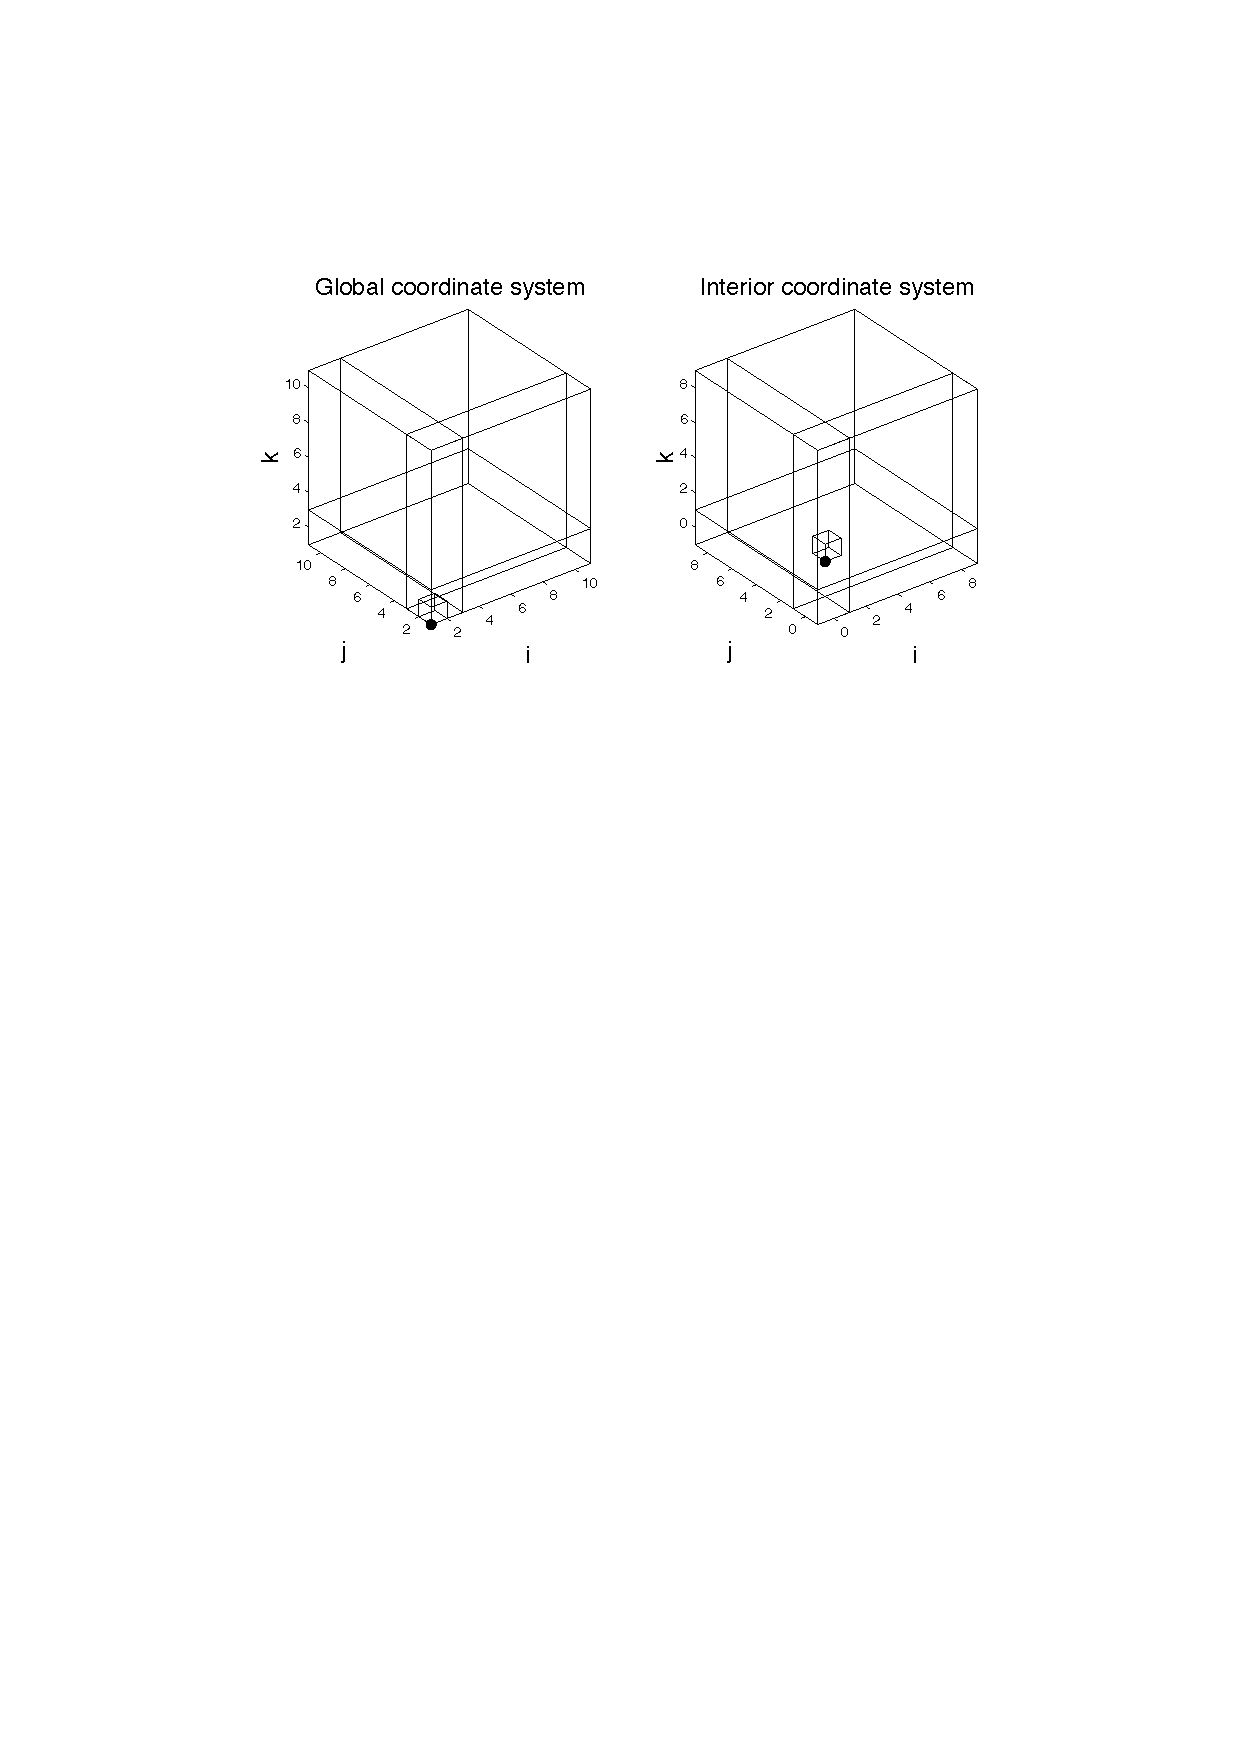
\includegraphics[width=\textwidth]{figures/0.pdf}
			\caption{FDTD global and interior coordinate systems. A PML of layer 2
				cells has been included on the lower side of the grid on each
				axis. The origin cell $(1,1,1)$ has been shown in each case}
			\label{fig:coords}
		\end{center}
	\end{figure}


	\subsection{Input File Format}
	The input file is written using the conventions of a matlab
	m-file. Thus, comments may be included using a \%. A number of values
	\emph{must} be specified in order for the FDTD program to execute. If a
	required value is not specified, the FDTD program will not execute but
	will report which value was not specified. The required input values
	are outlined below using the categories mentioned previously.

	\subsubsection{Grid}
	\begin{itemize}
		\item \verb+dimension+: This specifies the dimensionallity of the
		simulation. It can take the values \verb+'TE'+, \verb+'TM'+ and
		\verb+'3'+ which represent the TE, TM and three dimensionaly
		simulations respectively. The default value of is   \verb+3+ \verb+dimension+
		\item \verb+I+: The number of non-PML cells in the FDTD grid in the
		$x$-direction.
		\item \verb+J+: The number of non-PML cells in the FDTD grid in the
		$y$-direction.
		\item \verb+K+: The number of non-PML cells in the FDTD grid in the
		$z$-direction.
		\item \verb+multilayer+: A double array of dimension $1\times (N_l-1)$
		where $N_l$ is the number of layers in the multilayer
		structure. Each element of \verb+multilayer+ gives the index of the
		Yee cell along the $z$-direction of an interface. A simulation
		without a multilayer structure, ie, homogeneous space would have
		\verb+multilayer+ set to \verb+[]+. This is demonstrated in the
		example of Figure \ref{fig:multilayer}.\begin{figure}[h]
			\begin{center}
				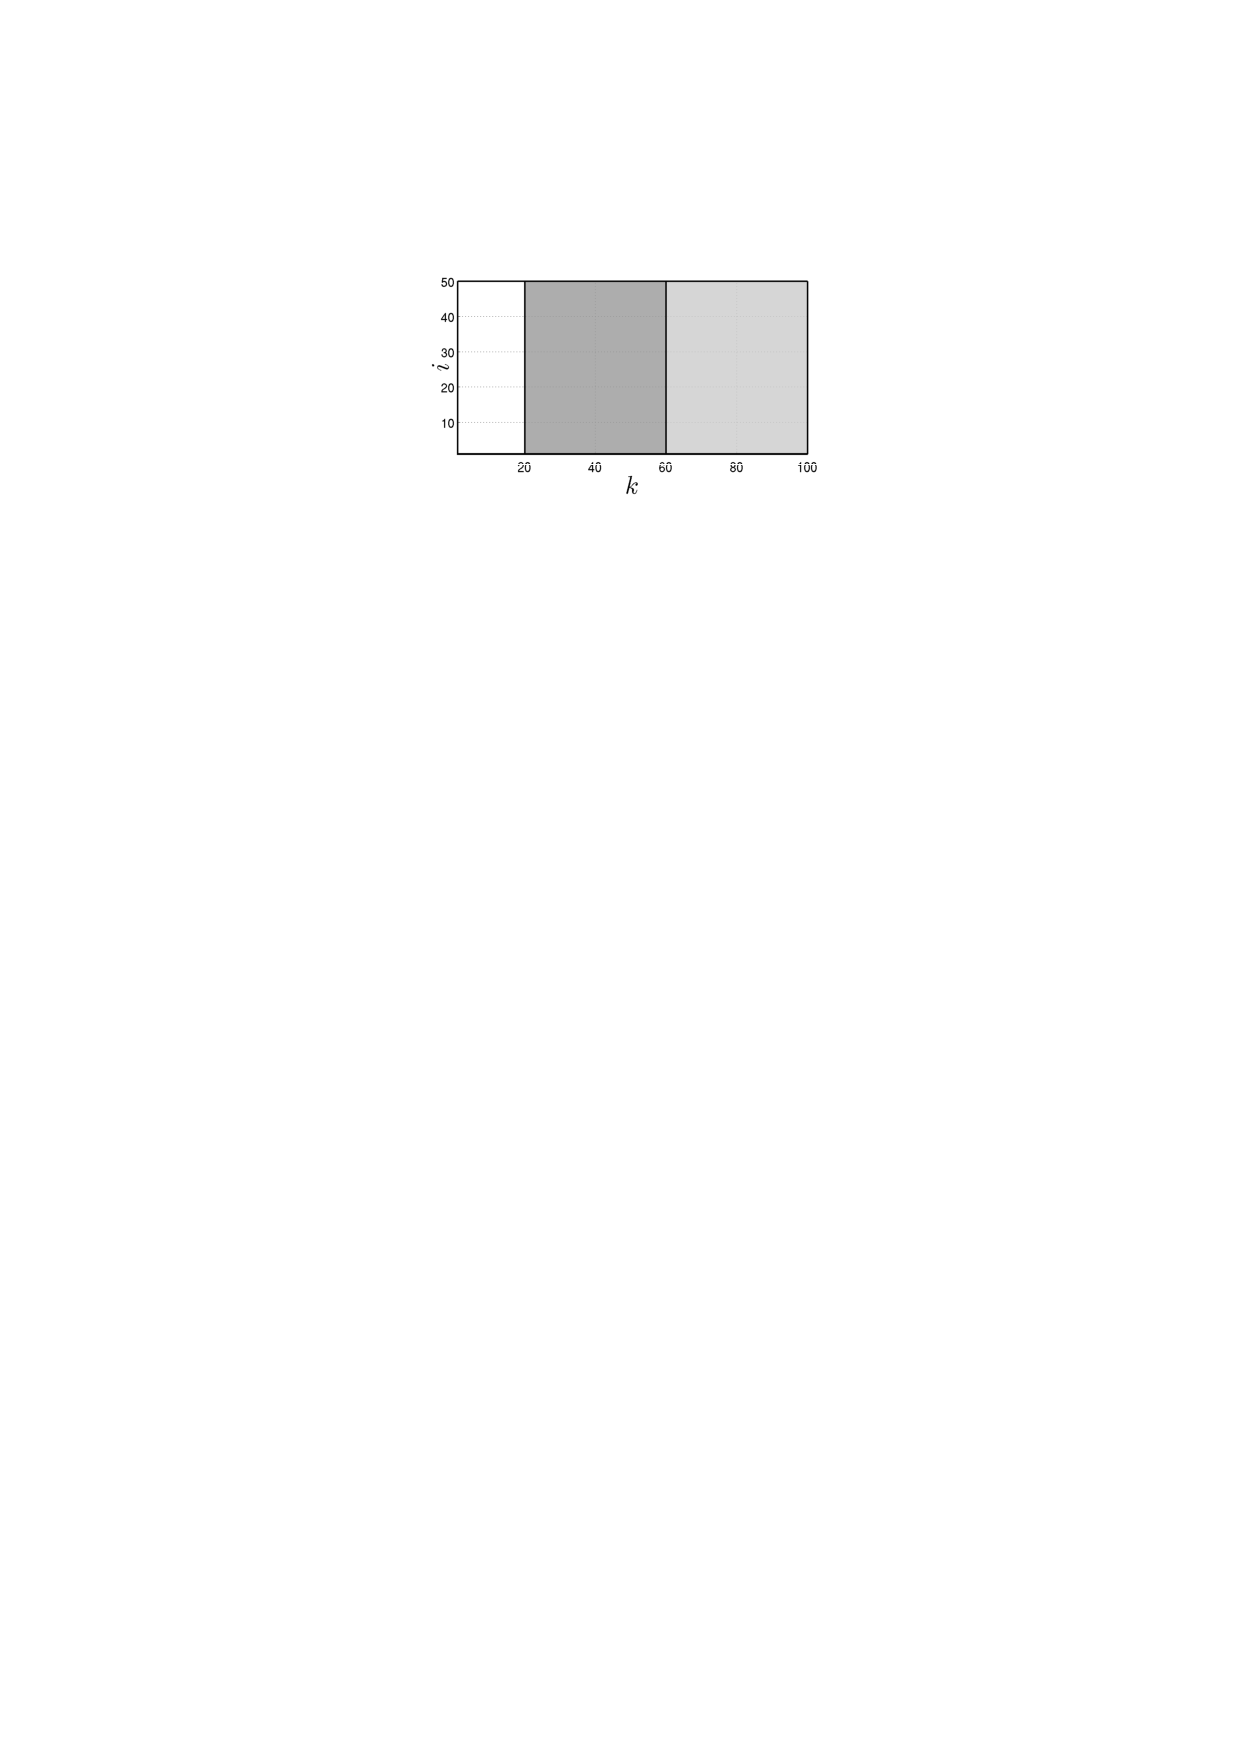
\includegraphics[width=\textwidth]{figures/1.pdf}
				\caption{Diagram showing the layers in a multilayer structure for the
					case of \texttt{multilayer=[24 40]} and therefore $N_l =3$.}
				\label{fig:multilayer}
			\end{center}
		\end{figure}
		\item \verb+epsr+: A  possibly complex vector of dimension $1\times
		N_l$ representing the non-dispersive relative permitivity of the background
		material which may be a multilayer structure.
		\item \verb+wp_vec+: A vector of dimension $1\times N_l$ which
		specifies the radian plasma frequency, $\omega_p$, of each
		layer. See Section \ref{sec:drude} for further details.
		\item \verb+vc_vec+: A vector of dimension $1\times N_l$ which
		specifies the collision frequency, $\nu_c$, of each layer. See
		Section \ref{sec:drude} for further details.

		\item \verb+mur+: The relative permeability of the background
		material. All cells in the grid are assumed to be composed of this
		material unless specified otherwise in the materials file. This is
		generally not varied from unity.
		\item \verb+structure+: A $2\times N$ matrix specifying the piece-wise
		linear profile of the multilayer structure when looking at the $xz$
		profile. Suppose that \verb+structure+ and \verb+multilayer+ are defined as:
		\begin{verbatim}
			structure = [i1 i2 ... iN;dk1 dk2 ... dkN];
			multilayer = [ki];
		\end{verbatim}
		then instead of having a plane interface at lattice coordinate $k1$,
		there is instead a piece-wise linear interface with vertices
		$(i1,ki+dk1)$, $(i2,ki+dk2)$, ..., $(iN,ki+dkN)$. Note that the
		structure is uniform along the j direction of the lattice.
		\item \verb+delta+: \emph{This should be set by someone with
			experience with FDTD and tested for suitability}. Describes the FDTD cell widths, must be a a matlab struct with the following members:
		\begin{itemize}
			\item \verb+delta.x+: Width of each FDTD cell in the $x$-direction
			(in m).
			\item \verb+delta.y+: Width of each FDTD cell in the $y$-direction
			(in m).
			\item \verb+delta.z+: Width of each FDTD cell in the $z$-direction
			(in m).
		\end{itemize}

		\item \verb+material_file+: This is the name of the file which
		describes the scattering object within the FDTD grid. This is
		explained in more detail in the accompanying ``FDTD
		material composition input file'' document. This is most often
		specified at the time calling the setup function in order to avoid
		having a large number of input files.
	\end{itemize}
	\subsubsection{Source}
	\begin{itemize}
		\item \verb+f_an+: The frequency in Hz of the incident electromagnetic
		field. This is the centre frequency of the source since the source
		is in general modulated by a Gaussian pulse.
		\item \verb+interface+: Describes where the incident field is
		introduced into the grid. Must be a matlab struct with the following
		members:
		\begin{itemize}
			\item \verb+interface.I0+: A $1\times 2$ vector where the first element
			gives the index $i$ of a plane parallel to the $jk$ plane where the
			incident field is introduced. The second element of the vector is a
			boolean value which determines whether or not the field will be
			introduced at the specified plane. The field will not be introduced
			if this is set to 0.
			\item \verb+interface.I1+: A $1\times 2$ vector where the first element
			gives the index $i$ of a plane parallel to the $jk$ plane where the
			incident field is introduced. The second element of the vector is a
			boolean value which determines whether or not the field will be
			intrduced at the specified plane. The field will not be introduced
			if this is set to 0.
			\item \verb+interface.J0+: A $1\times 2$ vector where the first element
			gives the index $j$ of a plane parallel to the $ik$ plane where the
			incident field is introduced. The second element of the vector is a
			boolean value which determines whether or not the field will be
			intrduced at the specified plane. The field will not be introduced
			if this is set to 0.
			\item \verb+interface.J1+: A $1\times 2$ vector where the first element
			gives the index $j$ of a plane parallel to the $ik$ plane where the
			incident field is introduced. The second element of the vector is a
			boolean value which determines whether or not the field will be
			intrduced at the specified plane. The field will not be introduced
			if this is set to 0.
			\item \verb+interface.K0+: A $1\times 2$ vector where the first element
			gives the index $k$ of a plane parallel to the $ij$ plane where the
			incident field is introduced. The second element of the vector is a
			boolean value which determines whether or not the field will be
			intrduced at the specified plane. The field will not be introduced
			if this is set to 0.
			\item \verb+interface.K1+ A $1\times 2$ vector where the first element
			gives the index $k$ of a plane parallel to the $ij$ plane where the
			incident field is introduced. The second element of the vector is a
			boolean value which determines whether or not the field will be
			intrduced at the specified plane. The field will not be introduced
			if this is set to 0.
		\end{itemize}
		\label{sec:cuboid}
		Six interface vectors are specified so that the incident field can be
		introduced on the surface of a cuboid. Inside the cuboid the total
		field is calculated and outside the cuboid the scattered field is
		calculate. Note that in most cases that we currently consider,
		\emph{only interface.K0 is required, the other interface
			conditions will be ignored}.  A diagram of a typical configuration
		is shown in Figure \ref{fig:interface}. The PML layers around the
		outer boundary have been included along with the interface
		plane. As shown in the right diagram (where some PML layers have been
		cut away), the interface plane marks the boundary between total and
		scattered field regions. The scattered field can always be recovered
		from the total field
		by subtracting the incident field from the total field.


		\begin{figure}[h]
			\begin{center}
				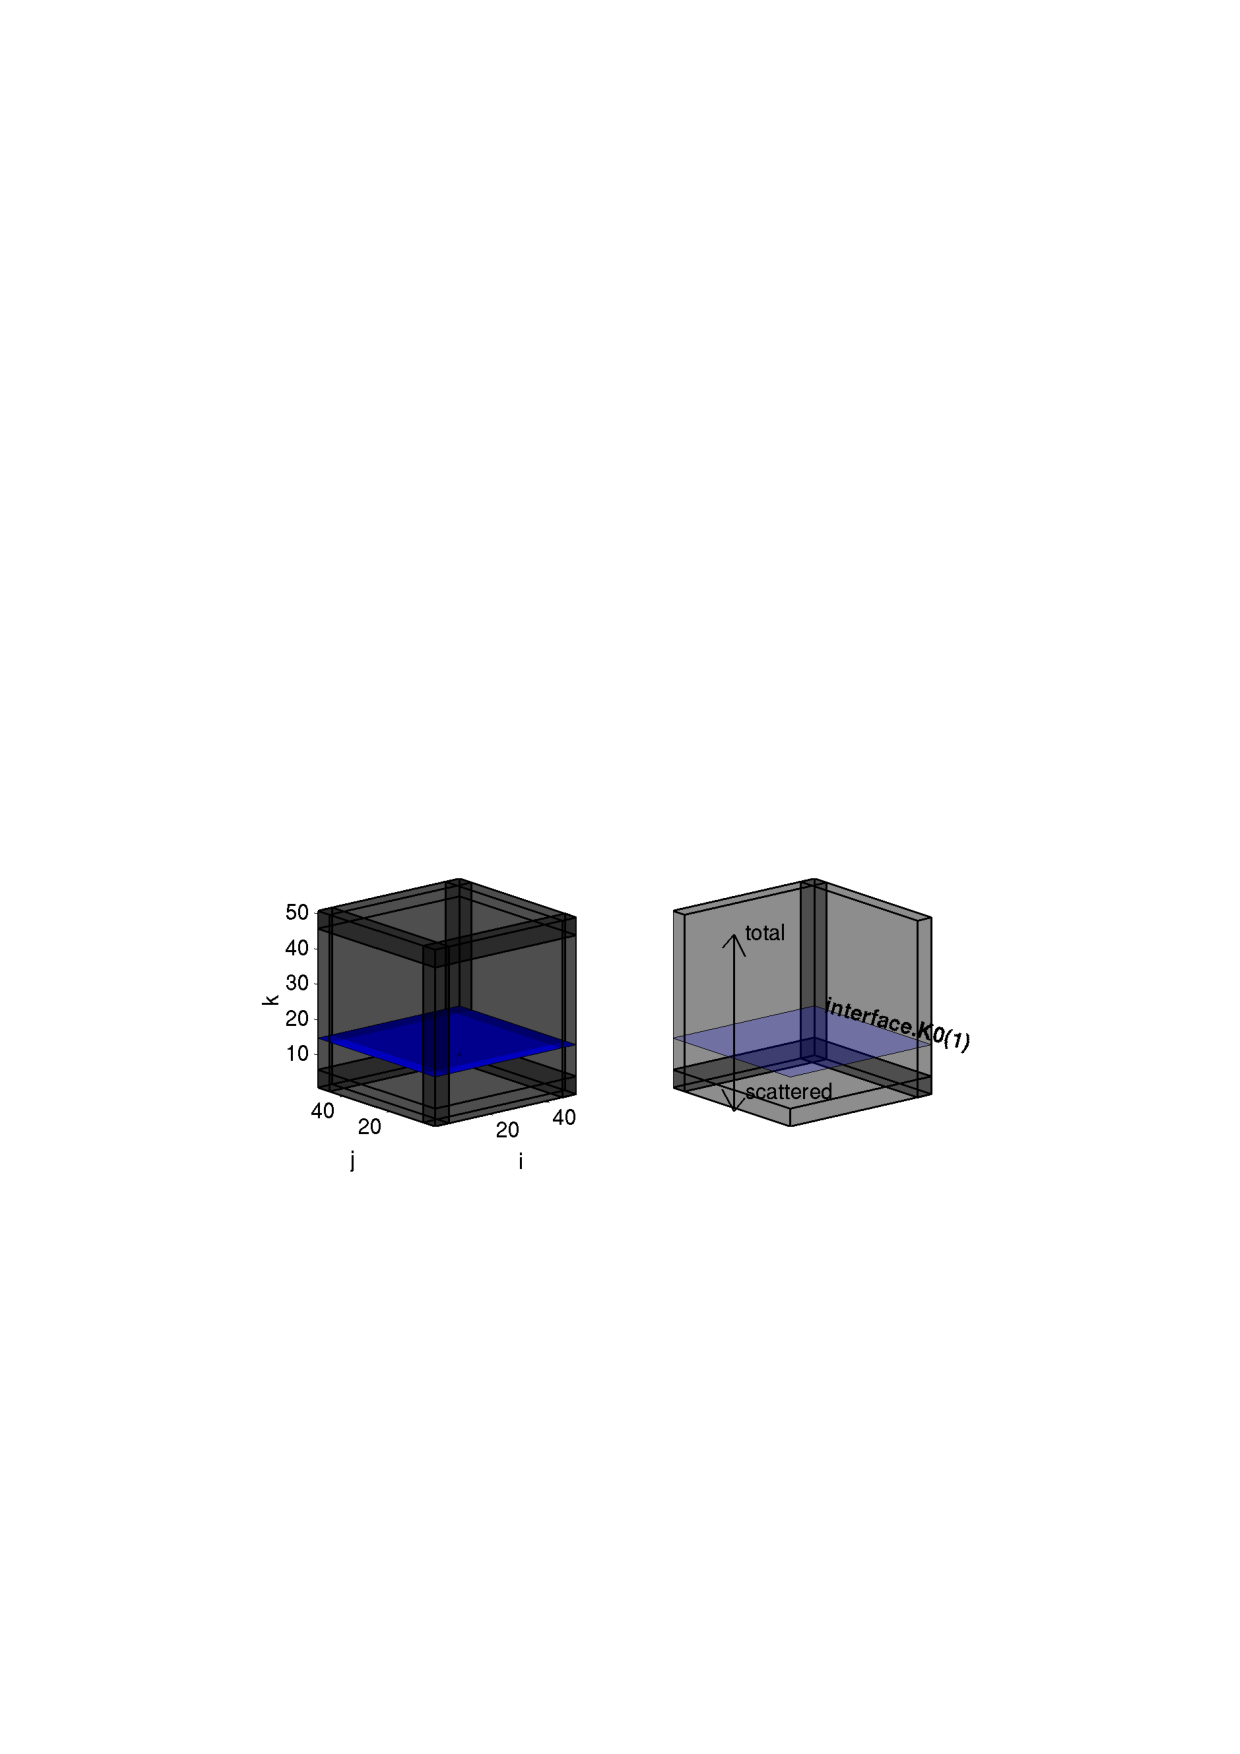
\includegraphics[width=\textwidth]{figures/2.pdf}
				\caption{Diagram of FDTD grid showing the PML and the interface
					plane. The right diagram the is same as the left except 3 of the PML
					layers have been cut away for clarity. The interface plane has been
					made partially transparent for clarity also.}
				\label{fig:interface}
			\end{center}
		\end{figure}

		\item \verb+efname+: The name of the m-file (as a string) which describes the
		incident electric field. The function should be structured
		as (where for example the line \verb+efname = 'plane_wave_electric'+
		appears in the input file):

		\begin{verbatim}
			function [E] = plane_wave_electric(X,Y,Z)
		\end{verbatim}

		Where:
		\begin{itemize}
			\item the parameters \verb+X+,\verb+Y+ and \verb+Z+ will be
			2-dimensional arrays similar in structure to that which  may be
			obtained by a call to matlab's \verb+meshgrid+ function. Note
			however that it should not be assumed that \verb+meshgrid+ has been
			employed. Values are passed with units of $ m$.
			\item \verb+E+ is a $1\times3$ cell array where \verb+E{1}+ contains
			the $x$-components of electric field, \verb+E{2}+ contains
			the $y$-components of electric field and \verb+E{3}+ contains
			the $z$-components of electric field.

		\end{itemize}
		Note that following relationship between the inputs
		\verb+X+,\verb+Y+ and \verb+Z+ and the output \verb+E+ must hold:
		\begin{eqnarray}
			E\{1\}(i,j)& =& E_x(X(i,j),Y(i,j),Z(i,j))  \nonumber \\
			E\{2\}(i,j)& =& E_y(X(i,j),Y(i,j),Z(i,j)) \nonumber \\
			E\{3\}(i,j)& =& E_z(X(i,j),Y(i,j),Z(i,j)) \nonumber
		\end{eqnarray}
		\emph{Also note that the field should obey the $\exp(-\imath \omega t)$ convention}.
		\item \verb+hfname+: The name of the m-file (as a string) which describes the
		incident magnetic field. This should have structure idential to that
		of the electric field function described above. \emph{Also note that
			the field should obey the $\exp(-\imath \omega t)$ convention}.
		\item \verb+illorigin+: Defines the cell which fixes the origin
		of the cartesian coordinate system of the FDTD grid. The incident
		electromagnetic field is defined relative to this coordinate
		system. For more information on this, see the section titled
		``Compuational space coordinate system'' in the accompanying ``FDTD
		material composition input file'' document.
		\item \verb+z_launch+: Sets the $z$-coordinate of the \verb+illorigin+
		cell. This cell will then have a position of $(0,0,z\_launch)$ in the
		cartesian coordinate system of the grid. The cartesian coordinates
		of other cells are found using the width of each FDTD cell. The
		cartesian coordinates are mapped to the interior FDTD lattice
		indices according to:
		\begin{equation}
			\left[\begin{array}{c} x\\ y\\ z\end{array}\right] = \left[\begin{array}{ccc}\Delta x & 0 & 0\\ 0 & \Delta y &
				0\\ 0 & 0 & \Delta z
			\end{array}\right]\left[\begin{array}{c}i-O_x\\j-O_y\\k-O_z\end{array}\right]+\left[\begin{array}{c} 0\\ 0\\ z_{launch}\end{array}\right]\label{eq:mapping}
		\end{equation}
		where \verb+illorigin+$=[O_x,O_y,O_z]$, \verb+z_launch+$=z_{launch}$
		and \verb+delta.x+$=\Delta x$ and so on for the other components.

		\item \verb+wavelengthwidth+: \emph{This parameter should be set by someone
			with experience in FDTD and should always be tested for
			suitability}. This is the spectral width of the modulating pulse of
		the incident electromagnetic field. The spectral width of this pulse
		should not be too wide as this will lead to the grid being unable to
		sufficiently spatially sample the field.
	\end{itemize}
	\subsubsection{Simulation type}
	\begin{itemize}
		\item \verb+sourcemode+: Specifies the type of source being
		employed. This may take the value \verb+'pulsed'+ or
		\verb+'steadystate'+. These options have the following meaning:
		\begin{itemize}
			\item \verb+'pulsed'+: This is the most commonly used method. It
			means that the incident electromagnetic field is introduced at a
			plane given by $k=interface.K0(1)$ and is introduced as a Gaussian
			pulse. A steady state response is calculated by taking a discrete
			Fourier transform at the required centre frequency (ie, that of
			the source) and accounting for the Fourier spectrum of the
			modulating pulse.
			\item
			\verb+'steadystate'+:
			This is when the incident electromagnetic field is gradually
			introduced and iteration continues until a steady state has been
			reached. When this option is used, the field around all faces of
			the interface cuboid must be specified (see section
			\ref{sec:cuboid}).
		\end{itemize}
		\item \verb+runmode+: This can take two values, \verb+'complete'+ or
		\verb+'analyse'+. These have the following meaning:
		\begin{itemize}
			\item \verb+'complete'+: Means the simulation will be run and phasors
			extracted and no time resolved information can be obtained from the
			simulation. This is the most common option. Note that this option
			must be used when the simulation is being run as a stand alone
			application (rather than being run from matlab).
			\item \verb+'analyse'+: Means the simulation will be run and the field
			at each iteration may be output to a file. This is useful for
			debugging or where it may be useful to view the field as it evolves
			in time. This option may only be used when the simulation is being
			run from matlab and not when it is being run as a stand alone application.
		\end{itemize}
	\end{itemize}
	\subsubsection{FDTD specific}
	These parameters should be set by an experienced FDTD user as they
	have a significant effect upon the accuracy of the simulation.
	\begin{itemize}
		\item \verb+dt+: This is the time step parameter used by the FDTD
		simulation. This is subject to the restriction \cite{taflove00book}:

		\begin{eqnarray}
			dt\le \frac{1}{c\sqrt{\frac{1}{delta.x^2}+\frac{1}{delta.y^2}+\frac{1}{delta.z^2}}}
		\end{eqnarray}
		However the program will automatically alter this if necessary. As a
		general guide, the time step should be chosen to be close to the
		upper limit as this will lead to a lower number of iterations
		required to complete the simulation.
		\item \verb+Nt+: The number of iterations to perform. This determines
		what period of time the FDTD simulates. Each iteration the FDTD
		simulation progresses by time \verb+dt+. When a \verb+'pulsed'+
		source is being used, the number of iterations
		must be set so that the field within the grid has decayed
		significantly. When a \verb+'steadystate'+ source is used the number
		of iterations must be dynamically set as a steady state must be
		reached before the simulation can end. In this case, \verb+Nt+ acts
		as an upper limit and the simulation will end if convergence is not reached.
	\end{itemize}
	\subsubsection{Output}
	These options control how the results of the simulation are output.
	\begin{itemize}
		\item \verb+outputs_array+: This enables various field components at
		selected points in the grid to be output at each iteration of the
		simulation. In general this should be set as \verb+outputs_array={}+
		as this option may only be used when \verb+runmode+ is set to
		\verb+'analyse'+. Each element of the cell array is itself a cell
		array with the following structure:
		\{filename,indextype,beginpoint,endpoint,components,writemethod\}
		where:
		\begin{itemize}
			\item \textbf{filename} is the name of the file or the base name used to
			write the data to.
			\item \textbf{indextype} can take the value \verb+'interior'+ or \verb+'global'+
			where in the former case the indices describing the range of cells
			to be output is given in interior coordinate system and in the
			latter case the global system is used (see Section
			\ref{sec:gridscheme}).
			\item \textbf{beginpoint} is a $1\times 3$ vector of indices giving
			the coordinate in the FDTD lattice of one vertex of a cuboid within
			which the field is output.
			\item \textbf{endpoint} is a $1\times 3$ vector of indices giving
			the coordinate in the FDTD lattice of the vertex of a cuboid within
			which the field is output. Note that in general this is diagonally
			opposite the beginpoint when is cuboid is specified, however by
			making some members of beginpoint and endpoint equal, the field on
			planes and lines can be extracted.
			\item \textbf{components} is a string containing one or more of the
			characters \verb+'x'+,\verb+'y'+ and
			\verb+'z'+.
			This is used to specify which field components are output.
			\item \textbf{writemethod} can be either
			\verb+'accumulate' or \verb+'dump'. In the former case a single mat
			file is written with all of the field data. In the latter case a
			separate fiel is written for each time increment.
		\end{itemize}

		%{'/tmp/fdtd_output3/6output','global',[60 1 1],[60 J+Dyl+Dyu+1 K+Dzl+Dzu+1],'xyz','dump'};
		\item \verb+exphasorsvolume+: Setting this to $1$ will cause phasors
		in the entire volume of the FDTD grid (excluding the PML) to be
		calculated. This leads to significantly more memory to be used but
		often provides useful information.
		\item \verb+exphasorssurface+: Setting this to $1$ will cause phasors
		to be extracted about the surface of a user specified cuboid. This
		is the most memory efficient way to extract the field and is all
		that is necessary for the general imaging model.
		\item \verb+phasorssurface+: Specifies the cuboid surface where the phasors
		should be extracted. Should be specified as:
		\begin{verbatim}
			phasorsurface = [i0 i1 j0 j1 k0 k1];
		\end{verbatim}
		Where \verb+i0+ is one of the faces of the cuboid parallel to the $jk$
		plane in the grid. \verb+i1+ is the other face of the cuboid parallel to the $jk$
		plane in the grid. Note that \verb+i0+ should be less than
		\verb+i1+. Similarly for the other indices. Figure \ref{fig:phasesurf}
		shows a sample mesh within an FDTD grid.
		\item \verb+phasorinc+: Often the spacing of vertices on the
		surrounding surface need not be as close as the Yee cell
		dimension. In this case it may be possible, depending on the lattice
		dimension, to skip some vertices. \verb+phasorinc+ is thus a
		$1\times 3$ dimensional vector of integers which divide their
		associated FDTD lattice dimension. That is, if
		\verb+phasorinc=[pix,piy,piz]+ then $pix$ should divide $I$ and
		$piy$ should divide $J$ etc. The default value of phasorinc is $[1,1,1]$.

		\begin{figure}[h]
			\begin{center}
				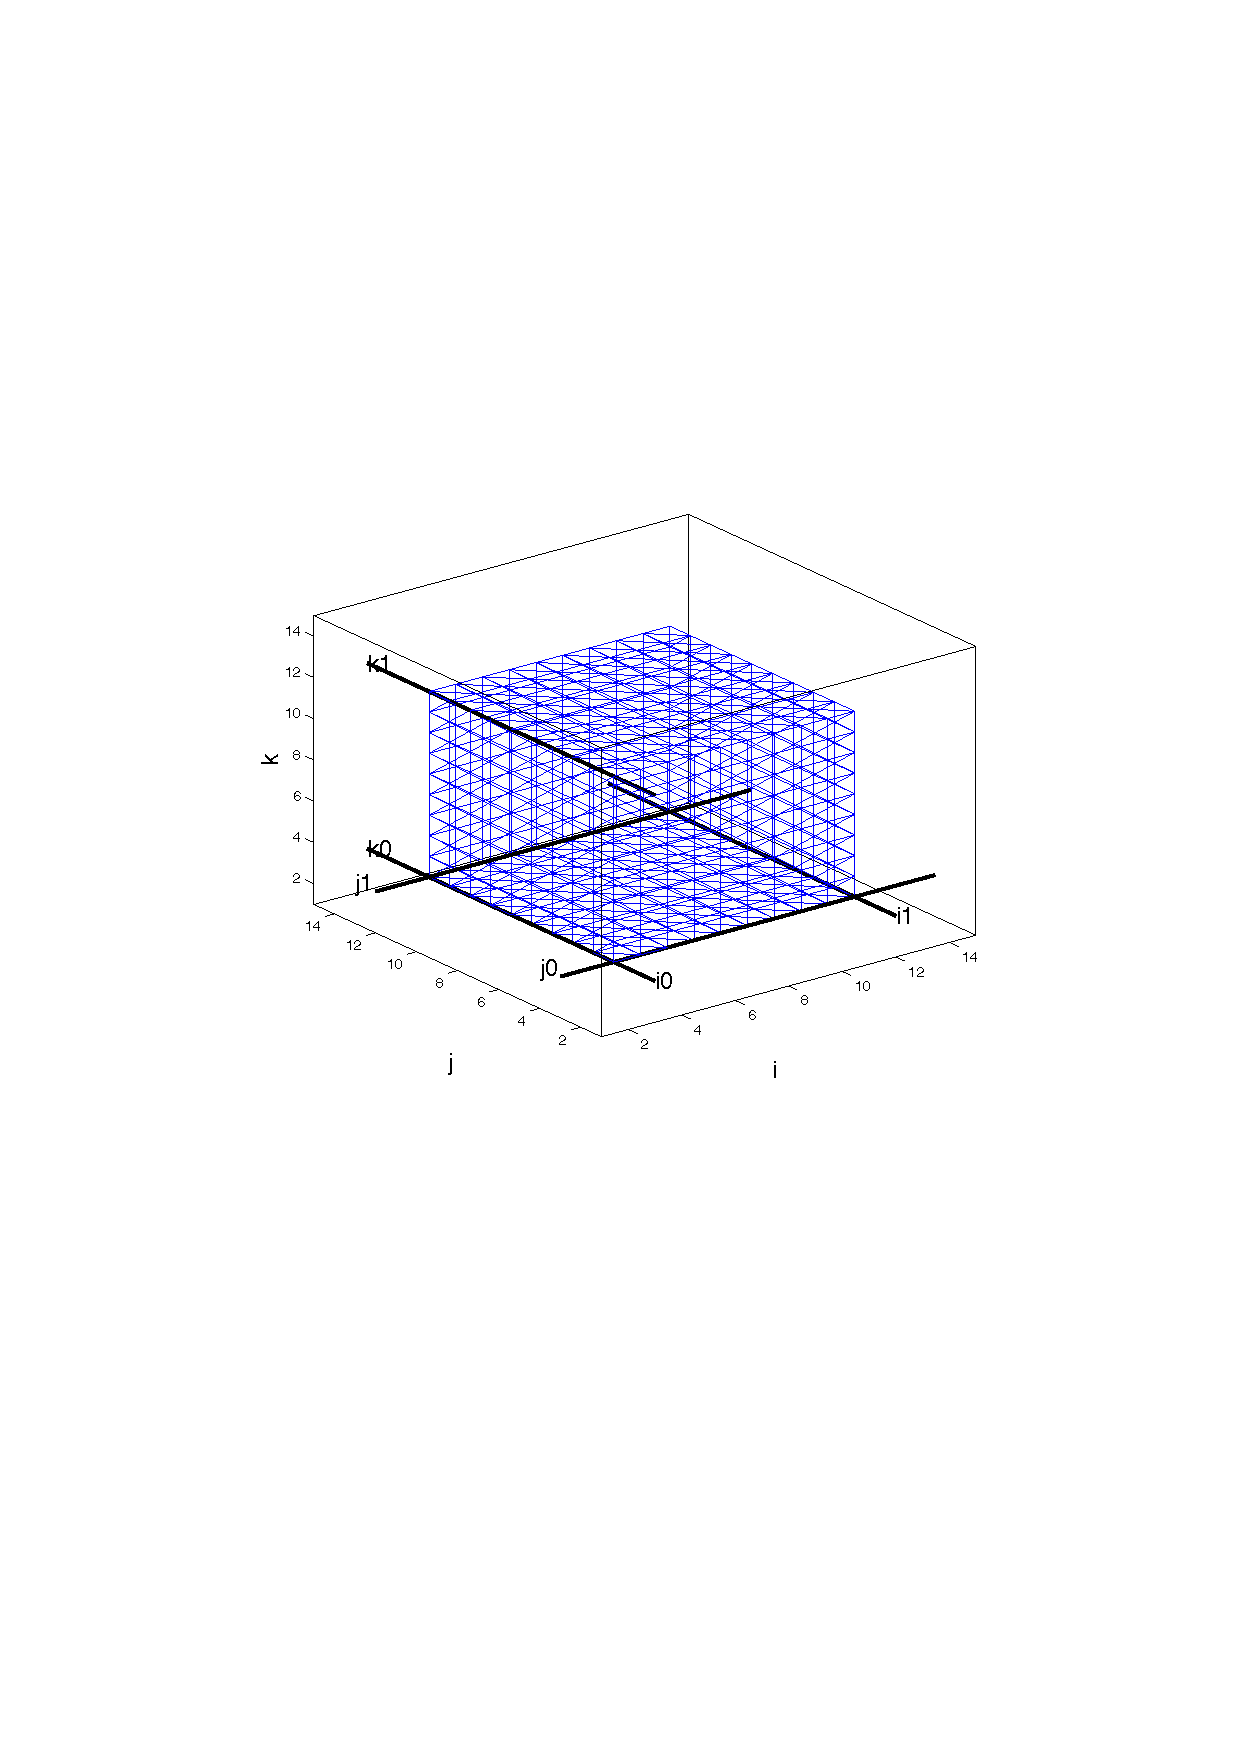
\includegraphics[width=\textwidth]{figures/3.pdf}
				\caption{Sample mesh within the FDTD grid illustrating the meaning of
					i0 to k1.}
				\label{fig:phasesurf}
			\end{center}
		\end{figure}


	\end{itemize}
	\subsubsection{PML}
	These parameters determine the properties of the PML. The PML is a
	layer of material which allows infinite scattering problems to be
	simulated using a finite grid. The PML acts as a very low reflection
	(theoretically zero), very high loss material. This any incident field
	is rapidly disipated with very small refelection. These should be set
	by an experienced user.
	\begin{itemize}
		\item \verb+n+: The order of the PML. The conductivity of the PML is
		increased at a rate proporional to $r^n$ where $r$ is the depth
		iside the PML. This is to reduce reflection due to numerical
		discretisation. The value depends upon what type of material is
		being terminated. A value of 2 works well for dielectric materials
		however a higher value has been shown to be effective for conducting
		and dispersive materials \cite{gedney96electromagnetics399,gedney96ieeetransantprop1630}.
		\item \verb+R0+ This is the maximum reflectiviy for a plane wave of
		arbitrary incidence. A value of $10^{-5}$ is often used successfully
		here. This should be tested particularly for the termination conductive and dispersive
		media.
		\item \verb+kappa_max+: When terminating conductive and dispersive
		materials it is necessary to have an additional parameter which
		varies with the same profile as the conductivity in the PML. It is
		set to 1 in the interior region. This maximum must be set through
		trial and error however Gedney has calculated some indicative values
		\cite{gedney96electromagnetics399,gedney96ieeetransantprop1630}. In
		the case of terminating dielectrics this should be set to 1. Thus,
		\verb+kappa_max+ is an $1\times N_i$ vector giving the value in each layer.
		\item \verb+Dxl+: The thickness of the PML in the $jk$ plane for cells
		having an $i$ index lower than that of the first non-PML cell in the
		$i$-direction.
		\item \verb+Dxu+: The thickness of the PML in the $jk$ plane for cells
		having an $i$ index greater than that of the last non-PML cell in
		the $i$-direction.
		\item \verb+Dyl+: The thickness of the PML in the $ik$ plane for cells
		having an $j$ index lower than that of the first non-PML cell in the
		$j$-direction.
		\item \verb+Dyu+: The thickness of the PML in the $ik$ plane for cells
		having an $j$ index greater than that of the last non-PML cell in
		the $j$-direction.
		\item \verb+Dzl+: The thickness of the PML in the $ij$ plane for cells
		having an $k$ index lower than that of the first non-PML cell in the
		$k$-direction.
		\item \verb+Dzu+: The thickness of the PML in the $ij$ plane for cells
		having an $k$ index greater than that of the last non-PML cell in
		the $k$-direction.
	\end{itemize}
	An example of how these variable relate to the PML widths is shown in
	Figure \ref{fig:pml}.
	\begin{figure}[h]
		\begin{center}
			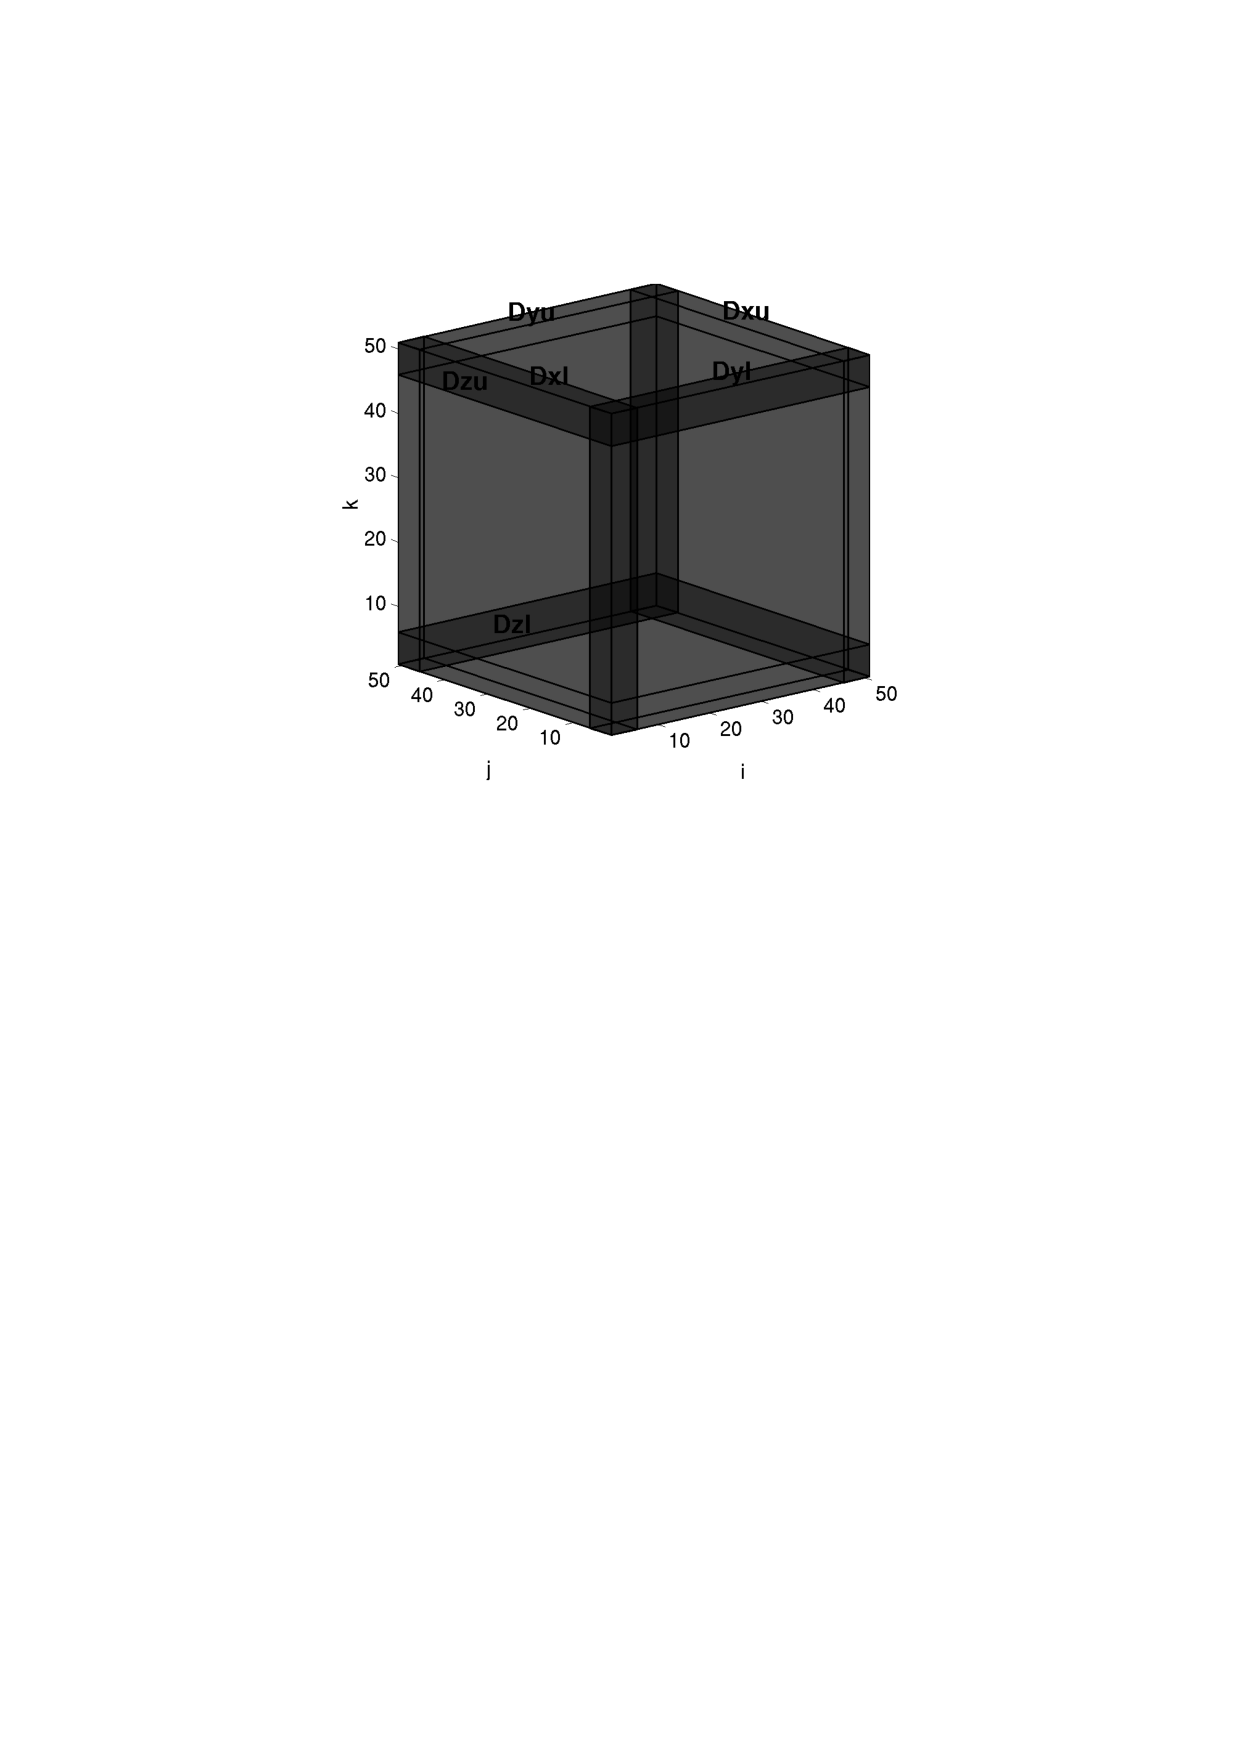
\includegraphics[width=\textwidth]{figures/4.pdf}
			\caption{Example of how the variables Dxl to Dzu specify the PML widths.}
			\label{fig:pml}
		\end{center}
	\end{figure}
	\section{Material file specification}
	The material file is used to specify the position and material type of
	scattering cells. Its definition draws heavily upon the mapping from
	the indexed space $\{(i,j,k)|1\le i\le I,1\le j\le J,1\le k\le K\}$ to
	the cartesian space as defined by Eq. \ref{eq:mapping}. The material
	file should be a \verb+.mat+ file with precisely two matrices named
	\verb+material_matrix+ and
	\verb+composition_matrix+. \verb+composition_matrix+ is an $N\times 4$
	array where N is the number of scattering cells. Each row of
	\verb+composition_matrix+ has the form:
	\begin{equation}
		\left[\begin{array}{llll} \textrm{material\_id}&i&j&k \end{array}\right]
	\end{equation}
	where $\textrm{material\_id}$ is an integer  denominating the
	type of material which makes up the scattering cell and is an index
	into the \verb+material_matrix+. The triple $(i,j,k)$ gives the
	position of the scattering cell represented by the matrix row. Each
	row of the \verb+material_matrix+ has the form:
	\begin{equation}
		\texttt{material\_matrix}=\left[\begin{array}{lllllllllll}\textrm{material\_id}
			& \epsilon_r & \mu_r & \nu_c & \omega_p & \sigma_x & \sigma_y &
			\sigma_z & \sigma_x^* & \sigma_y^* &
			\sigma_z^* \end{array}\right]
	\end{equation}
	where $\textrm{material\_id}$ is the integer identified of the
	material, $\epsilon_r$ is the real part of the relative permittivity and
	$\mu_r$ is the magnetic permeability. When using a dispersive material
	model $\nu_c$ is the collision
	fequency, $\omega_p$ is the radian plasma frequency. These should be
	set to 0 when not specifying a dispersive material. $\sigma_x$,
	$\sigma_y$, $\sigma_z$, $\sigma_x^*$, $\sigma_y^*$ and $\sigma_z^*$
	are the conductivities associated with the split formulation of
	Berenger's \cite{taflove00book}. In general, one should set
	$\sigma_x=\sigma_y=\sigma_z=\sigma$ to model a material with
	electrical conductivity $\sigma$.
	%<material identifier> <eps_r> <mu_r> <v_c> <w_p> <sigma_x> <sigma_y>
	%<sigma_z> <sigma_x*> <sigma_y*> <sigma_z*>
	\subsection{Dispersive Media}\label{sec:drude}
	Hitherto, we have not applied this model to the solution of time
	varying problems. Thus, unclusion of the Drude model is only to be
	able to model a general complex permitivity at a single
	frequency. Thus, it may be simpler to employ an expression the
	relative permitivity containing only a single pole however for a
	variety of reasons the full Drude model was implemented.

	Starting with the definition of complex permitivity according to
	Drude and assuming the $\exp(-i\omega t)$ time convention:
	\begin{equation}
		\epsilon_r=\epsilon_\infty - \frac{\omega_p^2}{\omega\left(\omega+i\nu_c\right)}\label{eq:drude}
	\end{equation}
	where $\omega_p$ is the plasma frequency and $\nu_c$ is the collision
	frequency. We can establish the relationship between the refractive
	index and various terms in Eq. \ref{eq:drude} according to:
	\begin{equation}
		\epsilon_r=(n_r+in_i)^2
	\end{equation}
	which yields:
	\begin{eqnarray}
		\nu_c&=&\frac{2n_in_r\omega}{\epsilon_\infty+n_i^2-n_r^2}\\
		\omega_p&=&\omega\sqrt{\epsilon_\infty+n_i^2-n_r^2+\frac{4n_i^2n_r^2}{\epsilon_\infty
				+ n_i^2 - n_r^2}}
	\end{eqnarray}
	These equations are sufficient to calculate $\omega_p$ and $\nu_c$ in
	order to obtain the desired relative permitivity at the radial frequency of
	interest $\omega$. Tests with the model suggest that a value of
	$\epsilon_\infty$ should be as close to unity as possible to obtain
	greater accuracy. The following section shows how the update equations
	in the non-PML part of the computational space are derived. More
	details can be obtained from Taflove and Hagness \cite{taflove00book}.
	\subsubsection{Derivation of update equations}
	Now we consider Ampere's law in the frequency domain:
	\begin{eqnarray}
		\nabla\times\boldsymbol{H}(\omega)=\sigma\boldsymbol{E}(\omega)-i\omega\epsilon_0\epsilon_r(\omega)\boldsymbol{E}(\omega)\label{eq:ampere}
	\end{eqnarray}
	Inverse Fourier transform easily casts the first two terms of this
	equation into the time domain however the final term is somewhat more
	complex. This may however be done according to:
	\begin{eqnarray}
		\mathfrak{F}^{-1}\left\{-i\omega\epsilon_0\epsilon_r(\omega)\boldsymbol{E}(\omega)\right\}&=&
		\epsilon_0\int_{-\infty}^{\infty}-i\omega\left(\epsilon_\infty -
		\frac{\omega_p^2}{\omega\left(\omega+i\nu_c\right)}\right)\boldsymbol{E}(\omega)\exp(-i\omega
		t)dt\\
		&=&\epsilon_0\epsilon_\infty\boldsymbol{E}'(t)+\boldsymbol{J}_p(t)
	\end{eqnarray}
	where
	\begin{eqnarray}
		\int_{-\infty}^{\infty}\omega\left(\omega+i\nu_c\right)\boldsymbol{J}_p(\omega)\exp(-i\omega t)dt&=&\epsilon_0\int_{-\infty}^{\infty}i\omega\omega_p^2\boldsymbol{E}(\omega)\exp(-i\omega
		t)dt\label{eq:jpexp1}
	\end{eqnarray}
	the left side of this expression yields
	\begin{eqnarray}
		\int_{-\infty}^{\infty}\omega\left(\omega+i\nu_c\right)\boldsymbol{J}_p(\omega)\exp(-i\omega
		t)dt&=&\int_{-\infty}^{\infty}\left(\omega^2+i\nu_c\omega\right)\boldsymbol{J}_p(\omega)\exp(-i\omega
		t)dt\\
		&=&\int_{-\infty}^{\infty}\left( -(-i\omega)^2 -\nu_c(-i\omega)\right)\boldsymbol{J}_p(\omega)\exp(-i\omega
		t)dt\\
		&=&-\boldsymbol{J}_p''(t) - \nu_c\boldsymbol{J}_p'(t)
	\end{eqnarray}
	the right hand side of Eq. \ref{eq:jpexp1} yields
	\begin{eqnarray}
		\epsilon_0\int_{-\infty}^{\infty}i\omega\omega_p^2\boldsymbol{E}(\omega)\exp(-i\omega
		t)dt&=&-\epsilon_0\omega_p^2\boldsymbol{E}'(t)
	\end{eqnarray}
	combining these results and eliminating the negative signs  yields
	\begin{eqnarray}
		\epsilon_0\omega_p^2\boldsymbol{E}'(t)=\boldsymbol{J}_p''(t) + \nu_c\boldsymbol{J}_p'(t)\label{eq:polarisationcurrent}
	\end{eqnarray}
	this expresses a relationship between the electric field strength
	vector and an auxilliary quantity, the so-called polarisation current
	${J}_p(t)$. We then express Eq. \ref{eq:polarisationcurrent} in terms
	of a discrete time step $\Delta t$ using central differences. This is
	done by making the substitutions:

	\begin{eqnarray}
		\epsilon_0\omega_p^2\left(\frac{\boldsymbol{E}^{n+1}-\boldsymbol{E}^{n-1}}{2\Delta
			t}\right)=\frac{\boldsymbol{J}_p^{n+1}-2\boldsymbol{J}_p^{n}+\boldsymbol{J}_p^{n-1}}{\Delta t^2}+\nu_c\left(\frac{\boldsymbol{J}_p^{n+1}-\boldsymbol{J}_p^{n-1}}{2\Delta
			t}\right)
	\end{eqnarray}
	which results in the following update equation:
	\begin{equation}
		\boldsymbol{J}_p^{n+1}=\alpha\boldsymbol{J}_p^{n}+\beta\boldsymbol{J}_p^{n-1}+\gamma\left(\frac{\boldsymbol{E}^{n+1}-\boldsymbol{E}^{n-1}}{2\Delta
			t}\right)\label{eq:jpmaster}
	\end{equation}
	where
	\begin{eqnarray}
		\alpha&=&\frac{4}{\nu_c\Delta t+2}\\
		\beta&=&\frac{\nu_c\Delta t-2}{\nu_c\Delta t+2}\\
		\gamma&=&\frac{2\epsilon_0\omega_p^2\Delta t^2}{\nu_c\Delta t+2}
	\end{eqnarray}
	Returning to Eq. \ref{eq:ampere} we can write the time domain
	expression for Ampere's law as
	\begin{eqnarray}
		\nabla\times\boldsymbol{H}(t)=\sigma\boldsymbol{E}(t)+\epsilon_0\epsilon_\infty\boldsymbol{E}'(t)+\boldsymbol{J}_p(t)
	\end{eqnarray}
	before proceeding to discretise this equation we must make the
	observation that if $\boldsymbol{E}(t)$ is known at time step $n$ then
	$\boldsymbol{H}(t)$ is known at time step
	$n+\frac{1}{2}$. Furthermore, $\boldsymbol{E}^{n+\frac{1}{2}}$ may be
	calculated according to
	$\boldsymbol{E}^{n+\frac{1}{2}}=\frac{1}{2}(\boldsymbol{E}^{n+1}+\boldsymbol{E}^{n})$.
	We can then write:
	\begin{eqnarray}
		\nabla\times\boldsymbol{H}^{n+\frac{1}{2}}&=&\sigma\frac{\boldsymbol{E}^{n+1}+\boldsymbol{E}^{n}}{2}+\epsilon_0\epsilon_\infty\frac{\boldsymbol{E}^{n+1}-\boldsymbol{E}^{n}}{\Delta
			t}+\frac{\boldsymbol{J}_p^{n+1}+\boldsymbol{J}_p^{n}}{2}\\
		&=&\sigma\frac{\boldsymbol{E}^{n+1}+\boldsymbol{E}^{n}}{2}+\epsilon_0\epsilon_\infty\frac{\boldsymbol{E}^{n+1}-\boldsymbol{E}^{n}}{\Delta
			t}+\nonumber\\&&+\frac{1}{2}\left[(1+\alpha)\boldsymbol{J}_p^{n}+\beta\boldsymbol{J}_p^{n-1}+\frac{\gamma}{2\Delta
			t}\left(\boldsymbol{E}^{n+1}-\boldsymbol{E}^{n-1}\right)\right]
	\end{eqnarray}
	rearrangement of the equations yields the update equation for
	$\boldsymbol{E}^n$ as:
	\begin{eqnarray}
		\boldsymbol{E}^{n+1}=C_a\boldsymbol{E}^n+C_c\boldsymbol{E}^{n-1}+C_b\Delta_i\left[\nabla\times\boldsymbol{H}^{n+\frac{1}{2}}-\frac{1}{2}\left((1+\alpha)\boldsymbol{J}_p^{n}+\beta\boldsymbol{J}_p^{n-1}\right)\right]\label{eq:masterfdtd}
	\end{eqnarray}
	where $\Delta_i$ refers to the Yee cell width in cartesian direction
	$i$, being $x$, $y$ or $z$.
	\begin{eqnarray}
		C_a&=&\frac{2\epsilon_\infty\epsilon_0-\sigma\Delta
			t}{2\epsilon_\infty\epsilon_0+\frac{1}{2}\gamma+\sigma\Delta t}\nonumber\\
		C_b&=&\frac{1}{\Delta_i}\frac{2\Delta
			t}{2\epsilon_\infty\epsilon_0+\frac{1}{2}\gamma+\sigma\Delta t}\nonumber\\
		C_c&=&\frac{1}{2}\frac{\gamma}{2\epsilon_\infty\epsilon_0+\frac{1}{2}\gamma+\sigma\Delta t}\label{eq:berengerC}
	\end{eqnarray}
	We now turn our attention to the discretisation of
	Eq. \ref{eq:masterfdtd} in space. There is more than possible indexing
	scheme for the Yee cell. One such example is shown in
	Fig. \ref{fig:yeediag}. Under this indexing scheme, the field
	component $E_x$ is located at position $(i+1/2,j,k)$ and similarly
	for the other field components. It is however simpler, and just as
	clear, to consider this field component as $E_x(i,j,k)$ and likewise
	for the other components. \begin{figure}[h]
		\centering
		% \includegraphics[width=.5\textwidth]{yee.eps}
		\caption{Diagram of a Yee cell showing how the various electromagnetic field
			components are sampled. The bolded cell shows the field components
			associated with cell $(i,j,k)$.}
		\label{fig:yeediag}
	\end{figure}In this way the curl part of Eq. \ref{eq:masterfdtd} is
	expanded as:
	\begin{eqnarray}
		\left(\nabla\times\boldsymbol{H}\right)_x&=&\frac{1}{\Delta_y}(H_z(i,j,k)-H_z(i,j-1,k))+\nonumber\\&&+\frac{1}{\Delta_z}(H_y(i,j,k-1)-H_y(i,j,k))\\
		\left(\nabla\times\boldsymbol{H}\right)_y&=&\frac{1}{\Delta_z}(H_x(i,j,k)-H_x(i,j,k-1))+\nonumber\\&&+\frac{1}{\Delta_x}(H_z(i-1,j,k)-H_z(i,j,k))\\
		\left(\nabla\times\boldsymbol{H}\right)_z&=&\frac{1}{\Delta_x}(H_y(i,j,k)-H_y(i-1,j,k))+\nonumber\\&&+\frac{1}{\Delta_y}(H_x(i,j-1,k)-H_x(i,j,k))
	\end{eqnarray}
	These equations thus permit the implementation of
	Eq. \ref{eq:masterfdtd}.
	\section{Output file format}
	The program writes the following variables into a \verb+.mat+ file:
	\begin{verbatim}
		Ex_out
		Ey_out
		Ez_out
		Hx_out
		Hy_out
		Hz_out
		x_out
		y_out
		z_out
		Ex_i
		Ey_i
		Ez_i
		Hx_i
		Hy_i
		Hz_i
		x_i
		y_i
		z_i
		vertices
		camplitudes
		facets
		maxresfield
	\end{verbatim}
	The meaning of each of these matrices is outlined below:
	\begin{itemize}
		\item \verb+Ex_out+, \verb+Ey_out+, \verb+Ez_out+, \verb+Hx_out+,
		\verb+Hy_out+ and \verb+Hz_out+ are complex amplitudes of the field
		defined within the non-PML FDTD lattice. Thus each field component is
		calculated at a different point in space as per the Yee cell. These
		are only calculated if \verb+exphasorsvolume+ is set to 1.
		\item \verb+x_out+, \verb+y_out+, \verb+z_out+ are the cartesian
		coordinates of the Yee cell origins of the fields specified in
		\verb+Ex_out+ etc. For example, the field component
		\verb+Ex_out(i,j,k)+ is associated with the Yee cell with origin
		positioned at
		$(\texttt{x\_out(i)},\texttt{y\_out(j)},\texttt{z\_out(k)})$.
		\item \verb+Ex_i+, \verb+Ey_i+, \verb+Ez_i+, \verb+Hx_i+,
		\verb+Hy_i+ and \verb+Hz_i+ are complex amplitudes of the field
		defined at the same points in space by using interpolation.
		\item \verb+x_i+, \verb+y_i+, \verb+z_i+ are the cartesian
		coordinates of positions where the field components \verb+Ex_i+ etc
		are defined. For example, the field component
		\verb+Ex_i(i,j,k)+ is located at position
		$(\texttt{x\_i(i)},\texttt{y\_i(j)},\texttt{z\_i(k)})$.
		\item \verb+vertices+ is an $N_v\times 3$ array of $N_v$ vertices where the
		time harmonic field has been extracted. This is only calculated if
		\verb+exphasorssurface+ is set to 1.
		\item \verb+camplitudes+ is an $N_v\times 6$ array of complex
		amplitudes, one for each vertex. Each row of the array has the form
		$(E_x,E_y,E_z,H_x,H_y,H_z)$.
		\item \verb+facets+ is an $N_f\times 3$ array of integers such that
		each row defines a facet. The union of all facets describes a cuboid
		defined in \verb+phasorsurface+. In general a mesh is represented by a set of vertices:
		$$\mathrm{V}=\left\{\mathbf{r}_{s,i}=\left(r_{s,i}^1,r_{s,i}^2,r_{s,i}^3\right)\in
		\mathbb{R}^3|1\le i\le N_v \right\}$$a set of facets:
		$$\mathrm{F}=\left\{\left(v^1_i,v^2_i,v^3_i\right)\in\mathbb{N}^3,1\le
		v_i^j\le N_v,1\le i\le N_f \right\}$$ where $N_v$ is the number of
		vertices and $N_f$ is the number of facets. The surface normal
		$\hat{\boldsymbol{n}}$ of facet $i$ is given by:
		$$\hat{\boldsymbol{n}}=\frac{(\mathbf{r}_{s,v^2_i}-\mathbf{r}_{s,v^1_i})\times(\mathbf{r}_{s,v^3_i}-\mathbf{r}_{s,v^1_i})}{|(\mathbf{r}_{s,v^2_i}-\mathbf{r}_{s,v^1_i})\times(\mathbf{r}_{s,v^3_i}-\mathbf{r}_{s,v^1_i})|}$$Note
		that this is an outward oriented surface normal.
		\item \verb+maxresfield+ is the maximum residual field in the FDTD
		lattice at the completion of the algorithm. This reveals whether
		a sufficient number of iterations have been executed in the case of a
		\verb+pulsed+ source.
	\end{itemize}
	\section{Compiling the executeable}
	You will probably receive the files as a gzipped tar file which can be
	extracted as:
	\begin{verbatim}
		$gunzip dispersive1.2.tar.gz
		$tar -xvf dispersive1.2.tar
	\end{verbatim}
	A make file is defined at
	\verb+dispersive/1.2/iterater/Makefile+. After setting the matlab root
	directory in the variable \verb+MATLABROOT+, the following commands
	should be sufficient to compile the executeable code:
	\begin{verbatim}
		$make clean
		$make
	\end{verbatim}

	\section{Running a simulation}
	\subsection{Problem setup}
	The m-file \verb+iteratefdtd_matrix+ is used to setup or run the FDTD
	simulation. It has the following options:
	\begin{verbatim}
		iteratefdtd_matrix(input_file,operation,outfile,material_file,ill_file)

		input_file    - file with input configuration information
		operation     - either 'run', 'filesetup', 'gridsetup' or
		'illsetup;. In the case of 'run', the FDTD
		simulation is completed. In the case of
		'filesetup', a mat file is written to file
		outfile. In the case of 'gridsetup' only the FDTD
		grid file is setup. In the case of 'illsetup' the illumination
		matrices are calculated and saved in matfile given by outfile.
		outfile       - the file that the above mentioned mat file is written to
		material_file - the material may be specified as an argument or in the
		input file. If it is specified by both, the one passed as a
		function argument is used.
		ill_file      - mat file containing the source field. Source will not
		be computed if this string is non empty.
	\end{verbatim}
	\subsection{Problem execution}
	A simulation may be executed using one of a number of possibilities as
	outlined below:
	\begin{verbatim}
		Usage: openandorder [options] infile outfile
		openandorder [options] infile gridfile outfile
		Options:
		-h:     Display this help message
		-m:     Minimise output file size by not saving vertex and facet information
	\end{verbatim}
	When a number of simulations are performed using the same simulation
	parameters with the exception of the scattering cells it is more
	efficient to specify the scattering cells seaprately in \verb+gridfile+.
	\section{Examples}
	The samples are in the directory
	\verb+dispersive1.2/doc/master/samples+.
	\subsection{Scattering of a plane wave by a dielectric sphere (case1)}
	This example calculates the light scattered by a sphere of refractive
	index 1.2 for an incident plane wave polarised in the y-direction. In order to create the input file, add \verb+dispersive1.2+ to the
	path. In particular, assuming the durrent directory is
	\verb+dispersive1.2/doc/master/samples+, the directory may be added
	using the command \verb+addpath('../../../');+. The input file,
	\verb+input_file_sphere_case1.m+ is listed below:
	\small
	\verbatiminput{samples/input_file_sphere_case1.m}
	\normalsize
	the input \verb+.mat+ file is then created by calling
	\verb+gen_input_sphere_case1+ from the matlab prompt. This file is
	listed below:
	\tiny
	\verbatiminput{samples/gen_input_sphere_case1.m}
	\normalsize
	This results in the following output from matlab:
	\small
	\verbatiminput{samples/case1.txt}
	\normalsize
	This output shows that since this example does not use certain
	features which are available, and the inputs corresponding to these
	features have not been set, the m-file has set them to their default
	values. Also, note that two \verb+.mat+ files have been produced, one
	which is the actual scattering calculation and one which calculates
	the free space propagation of the incident wave. Note that although
	the incident wave is known analytically, the one which propagates in
	the FDTD computational space can very slightly due to numerical
	dispersion. The result of these scattering calculations are calculated
	according to:

	\begin{verbatim}
		$../../../iterater/prtmfdtd case1_fs.mat case1_fs_out.mat
		$../../../iterater/prtmfdtd case1.mat case1_out.mat
	\end{verbatim}

	Finally, the result can be compared to the field calculated using the
	series of Mie by executing \verb+analyse_res_case+, resulting in the
	results displayed in Figure .

	\begin{figure}[!h]
		\begin{center}
			% \includegraphics[bb=0 0 934 700,width = .7\textwidth]{samples/case1_comparison.jpg}\label{fig:case1}
			\caption{Comparison between FDTD and Mie results for a dielectric
				sphere in air with relative permitivity 1.2. FDTD results are
				displayed on the top row.}
		\end{center}
	\end{figure}
	The error may be calculated according to:
	\begin{equation} \label{e:Global-Error-Metric-copy}
		\epsilon_\mathbf{E}^\mathbf{s}=\frac{\sum_{i=1}^{N}|{\mathbf{E}^{fdtd}(\mathbf{r}_{i})\cdot\mathbf{s}-\mathbf{E}^{mie}(\mathbf{r}_{i})\cdot\mathbf{s}}|^{2}}%
		{\sum_{i=1}^{N}|\mathbf{E}^{mie}(\mathbf{r}_{i})\cdot\mathbf{s}|^{2}}
	\end{equation}
	where $N$ is the number of points where the field is
	sampled, $\mathbf{E}^{fdtd}$ is the field calculated using the FDTD method, $\mathbf{E}^{mie}$ is the field
	calculated using Mie theory, $\mathbf{r}_i$ is the position of the
	$i$th field value and $\mathbf{s}$ is the component of the field to
	consider. The error is calculated as:
	\newline
	\begin{table}[hbp]
		\begin{tabular}{|c|c|c|c|}
			\hline
			&$\mathbf{\hat{i}}$&$\mathbf{\hat{j}}$&$\mathbf{\hat{k}}$\\
			\hline
			$\mathbf{E}$&0.0193&    0.0194&    0.0193\\
			$\mathbf{H}$&0.0194&    &    0.0194\\
			\hline
		\end{tabular}
	\end{table}
	note that $\epsilon_\mathbf{H}^\mathbf{\hat{j}}$ is not given as there
	is an error in calculating the y component of the magnetic field.
	\subsection{Further examples of scattering of a plane wave by a
		sphere}
	Further examples have been constructed where the refractive index of
	the sphere is varied. There are examples where conductivity is used to
	obtain a complex refractive index and also where a dispersive model is
	used. Table summarises the properties of each example.

	\begin{table}[!h]
		\begin{center}
			\begin{tabular}{|c|c|c|c|}
				\hline
				m-file&n$_{sphere}$&model type&radius\\
				\hline
				\verb+gen_input_sphere_case1.m+&1.2&dielectric&$\lambda/8$\\
				\hline
				\verb+gen_input_sphere_case2.m+&1.2020 + 0.0701i&conductive&$\lambda/8$\\
				\hline
				\verb+gen_input_sphere_case3.m+&1.2020 + 0.0701i&dispersive&$\lambda/8$\\
				\hline
				\verb+gen_input_sphere_case4.m+&0.5020 + 4.9200i&dispersive&$\lambda/8$\\
				\hline
				\verb+gen_input_sphere_case5.m+&0.5020 + 4.9200i&dispersive&$\lambda/4$\\
				\hline
			\end{tabular}
		\end{center}
		\caption{Summary of sphere scattering examples.}
		\label{tab:examples}
	\end{table}

	Each of these results can be analysed by setting the value of
	\verb+sphere_case+ in the m-file \verb+analyse_res_case.m+ and
	executing the m-file.
	\subsection{Reflection by a conducting medium}
	A further example is given where reflection of a plane wave by a plane
	conducting surface normal to the direction of propagation is
	calculated. The input file is generated by the m-file
	\newline\verb+dispersive1.2/doc/master/samples/multi_layer/gen_input_disp.m+
	and the result analysed by the m-file \verb+calc_ref.m+.

	\subsection{Diffraction by a circular aperture}
	The m-file
	\newline\verb+dispersive1.2/doc/master/samples/multi_layer/gen_input_ap.m+
	generates an input file which may be used to calculate the diffraction
	by a circular aperture in a conducting medium of finite thickness and conductivity.

	\bibliography{refs}
	\clearpage

	\appendix
	\section{The finite-difference time-domain method}
	\subsection{Overview}
	\label{sec:numermeth:fdtd}
	The FDTD method differs appreciably
	from the methods discussed previously. All methods mentioned thus far
	are frequency domain methods and solve a boundary value problem. The
	FDTD method works in the time domain and solves an initial value
	problem. It literally models the evolution, over time, of a field
	incident upon a scatterer and the resulting scattered field. The
	method is attributed to Yee \cite{yee66ieeetransantprop302} who
	published the seminal paper on the FDTD method in 1966 although it
	was not applied in three dimensions until 1975 by Taflove
	\cite{taflove75ieeetransmicrotheoryandtech623,taflove75ieeetransmicrotheoryandtech888}.
	Since the publication of these papers, the method has developed
	immensely and is now a very mature numerical method used in numerous
	applications.

	The starting point of the FDTD method is two of Maxwell's equations in the
	time domain:
	\begin{eqnarray}
		\label{eq:numermeth:maxtime1}
		\nabla\times\mathbf{E}&=&-\frac{\partial\mathbf{B}}{\partial t}-\sigma^*\mathbf{H}\\
		\label{eq:numermeth:maxtime2}
		\nabla\times\mathbf{H}&=&\mathbf{J} + \frac{\partial\mathbf{D}}{\partial t}
	\end{eqnarray}
	where $\sigma^*$ is the equivalent magnetic loss ($\Omega$/m) which is
	required in the analysis of PMLs. Each of these equations yields a set of coupled partial differential
	equations. For example, by using the constitutive relationships
	stated in \eq{fig:numermeth:constituteb}:
	\begin{eqnarray}
		\label{fig:numermeth:constituted}
		\mathbf{D}&=&\epsilon_r\epsilon_0\mathbf{E}\\
		\mathbf{B}&=&\mu_r\mu_0\mathbf{H}
		\label{fig:numermeth:constituteb}
	\end{eqnarray}
	where:\\
	$\epsilon_r$ is the relative permittivity\\
	$\epsilon_0$ is the permittivity of free space\\
	$\mu_r$ is the relative permeability, and\\
	$\mu_0$ is the permeability of free space\\\\
	and also by making the substitution
	$\mathbf{J}=\mathbf{J}_{source}+\sigma\mathbf{E}$ where
	$\mathbf{J}_{source}$ represents a source of current density and
	$\sigma$ is the material conductivity, the
	following partial differential equation is obtained from \eq{eq:numermeth:maxtime2}:
	\begin{equation}
		\frac{\partial E_x}{\partial
			t}=\frac{1}{\epsilon_r\epsilon_0}\left[\frac{\partial H_z}{\partial
			y} - \frac{\partial H_y}{\partial z} - \left({J_{source_x}}+\sigma E_x\right)\right]
		\label{eq:numermeth:pde}
	\end{equation}
	Yee's objective when developing the FDTD method was to discretise
	the coupled set of partial differential equations. Derivatives become
	differences during this process. One of the key features of the FDTD
	method is that it employs a central differencing scheme which
	achieves second order accuracy. To understand the concept of central
	differences, consider calculating the first derivative of a function
	$f(x)$ using only a difference equation. By expanding $f$ in
	a Taylor series about $x_i$, it is possible to write:
	\begin{eqnarray}
		f(x_i\pm\Delta x)&=&f(x_i)\pm\Delta xf'(x_i)+\frac{\Delta x^2}{2!}f''(x_i)
		\pm \frac{\Delta x^3}{3!}f'''(x_i) + \ldots\label{eq:numermeth:fxplus}\\
		\label{eq:numermeth:fxminus}
	\end{eqnarray}
	Subtracting $f(x_i-\Delta x)$ from $f(x_i+\Delta x)$ yields the following expression:
	\begin{equation}
		f(x_i+\Delta x)-f(x_i-\Delta x) = 2f'(x_i)\Delta x
		+\frac{2\Delta x^3}{3!}f'''(x_i) + \ldots
		\label{eq:numermeth:centdiff1}
	\end{equation}
	after dividing by $2\Delta x$, this gives $f'(x_i)$ as
	\begin{equation}
		f'(x_i)=\frac{f(x_i+\Delta x) - f(x_i-\Delta x)}{2\Delta x}+O(\Delta x^2)
		\label{eq:numermeth:centdiff}
	\end{equation}
	This is called a central difference operation as the derivative of $f$
	may be approximated at a point which is in the centre of two
	points where the value of the function is known. The partial differential equations obtained from Maxwell's equations
	have both spatial and temporal derivatives. This means that special
	care must be taken when constructing the computational grid in order
	to facilitate spatial central differences and also when choosing the
	time stepping scheme to allow temporal central differencing. The FDTD simulation employs a regular grid of
	points where the various electromagnetic field components are
	sampled. The grid is built up through periodic replication of the
	Yee cell (see \rfig{fig:numermeth:yeediag}). The position of a
	particular point within
	the grid is denoted by a triple of indices $(i,j,k)$ which corresponds
	to position $(i\Delta_x,j\Delta_y,k\Delta_z)$ where $\Delta_x$,
	$\Delta_y$ and $\Delta_z$ are the lengths of the Yee cell in the $x$,
	$y$- and $z$-directions respectively. Time is also discretised and
	referred to using a single increment $n$ which corresponds to the
	simulation time $n\Delta t$ where $\Delta t$ is the time increment
	being used in the simulation. Thus the $x$-component of the electric
	field at position $(i,j+1/2,k+1/2)$ and time $n-1/2$ may be denoted by
	$E_x|^{n-1/2}_{i,j+1/2,k+1/2}{\Delta t}$.Using this notation, \eq{eq:numermeth:pde} may be
	written as \cite{taflove00book}:
	\begin{align}
		\frac{E_x|^{n+1/2}_{i,j+1/2,k+1/2}-E_x|^{n-1/2}_{i,j+1/2,k+1/2}}{\Delta
			t}&=\nonumber\\
		\frac{1}{\epsilon_0\epsilon_{r_{i,j+1/2,k+1/2}}}&\left(\begin{array}{c}\frac{H_z|^n_{i,j+1,k+1/2}-H_z|^n_{i,j,k+1/2}}{\Delta
				y}-\\ \frac{H_y|^n_{i,j+1/2,k+1}- H_y|^n_{i,j+1/2,k}}{\Delta z}-\\ {J_{source_x}}|^n_{i,j+1/2,k+1/2}-\\\sigma_{i,j+1/2k+1/2}E_x|^n_{i,j+1/2,k+1/2}\end{array}\right)
		\label{eq:numermeth:difference1}
	\end{align}
	It is noted from these equations that each $E_x$ component must be
	positioned midway between two $H_y$ and two $H_z$ components. To
	proceed further a semi-implicit approximation must be used to replace
	the $E_x|^n_{i,j+1/2,k+1/2}$ term in \eq{eq:numermeth:difference1} with:
	\begin{equation}
		E_x|^n_{i,j+1/2,k+1/2}=\frac{E_x|^{n+1/2}_{i,j+1/2,k+1/2} + E_x|^{n-1/2}_{i,j+1/2,k+1/2}}{2}
		\label{eq:numermeth:semiimp}
	\end{equation}
	Resulting in the expression:
	\begin{align}
		E_x|^{n+1/2}_{i,j+1/2,k+1/2}=C_a|_{i,j+1/2,k+1/2}&E_x|^{n-1/2}_{i,j+1/2,k+1/2}+\nonumber\\
		C_b|_{i,j+1/2,k+1/2}&\left(\begin{array}{c}H_z|^n_{i,j+1,k+1/2} -
			H_z|^n_{i,j,k+1/2}+\\H_y|^n_{i,j+1/2,k}-H_y|^n_{i,j+1/2,k+1}-\\{J_{source_x}}|^n_{i,j+1/2,k+1/2}\Delta\end{array}
		\right)
	\end{align}
	where $C_a$ and $C_b$ are functions of $\epsilon_r$, $\sigma$, $\Delta
	t$, $\Delta$ and position within the FDTD grid and it is assumed
	that $\Delta x$=$\Delta y$=$\Delta z$=$\Delta$. Each of the partial differential
	equations like \eq{eq:numermeth:pde} may be converted into a
	difference equation in the same manner. The result of this is a system
	of equations where the $\mathbf{E}$ and $\mathbf{H}$ fields can be
	advanced by a time step at each iteration from an initial set of field
	values. Note that that in order to facilitate central differences in
	time, the $\mathbf{E}$ and $\mathbf{H}$ fields are calculated half a
	time step apart.

	The difference equations also dictate a particular arrangement of
	field components within the computational grid proposed by Yee. The
	arrangement and the basic cell used to demonstrate this arrangement is
	known as the Yee cell and is shown in \rfig{fig:numermeth:yeediag}. It
	shows that the field components are offset from one another so as to
	allow the central difference equations to work correctly. Another
	important property of the Yee cell is its suitability to the
	application of PEC boundary conditions. On a PEC boundary the
	tangential component of electric field and normal component of
	magnetic field vanish. Thus a PEC boundary is easily imposed upon any
	of the faces of the Yee cell.

	As previously mentioned, the FDTD method essentially solves an initial
	value problem. In most problems however, a known field is incident upon
	the scattering object for a period comparable to the simulation time. In order to deal with this the FDTD grid is
	divided up into two regions. One region surrounds the scatterer and
	the total field is calculated in this region. Only the scattered field
	is calculated in the scattered region. This is very similar to the
	partitioning illustrated in \rfig{fig:numermeth:scat_tot}. \begin{figure}[!h]
		\centering
		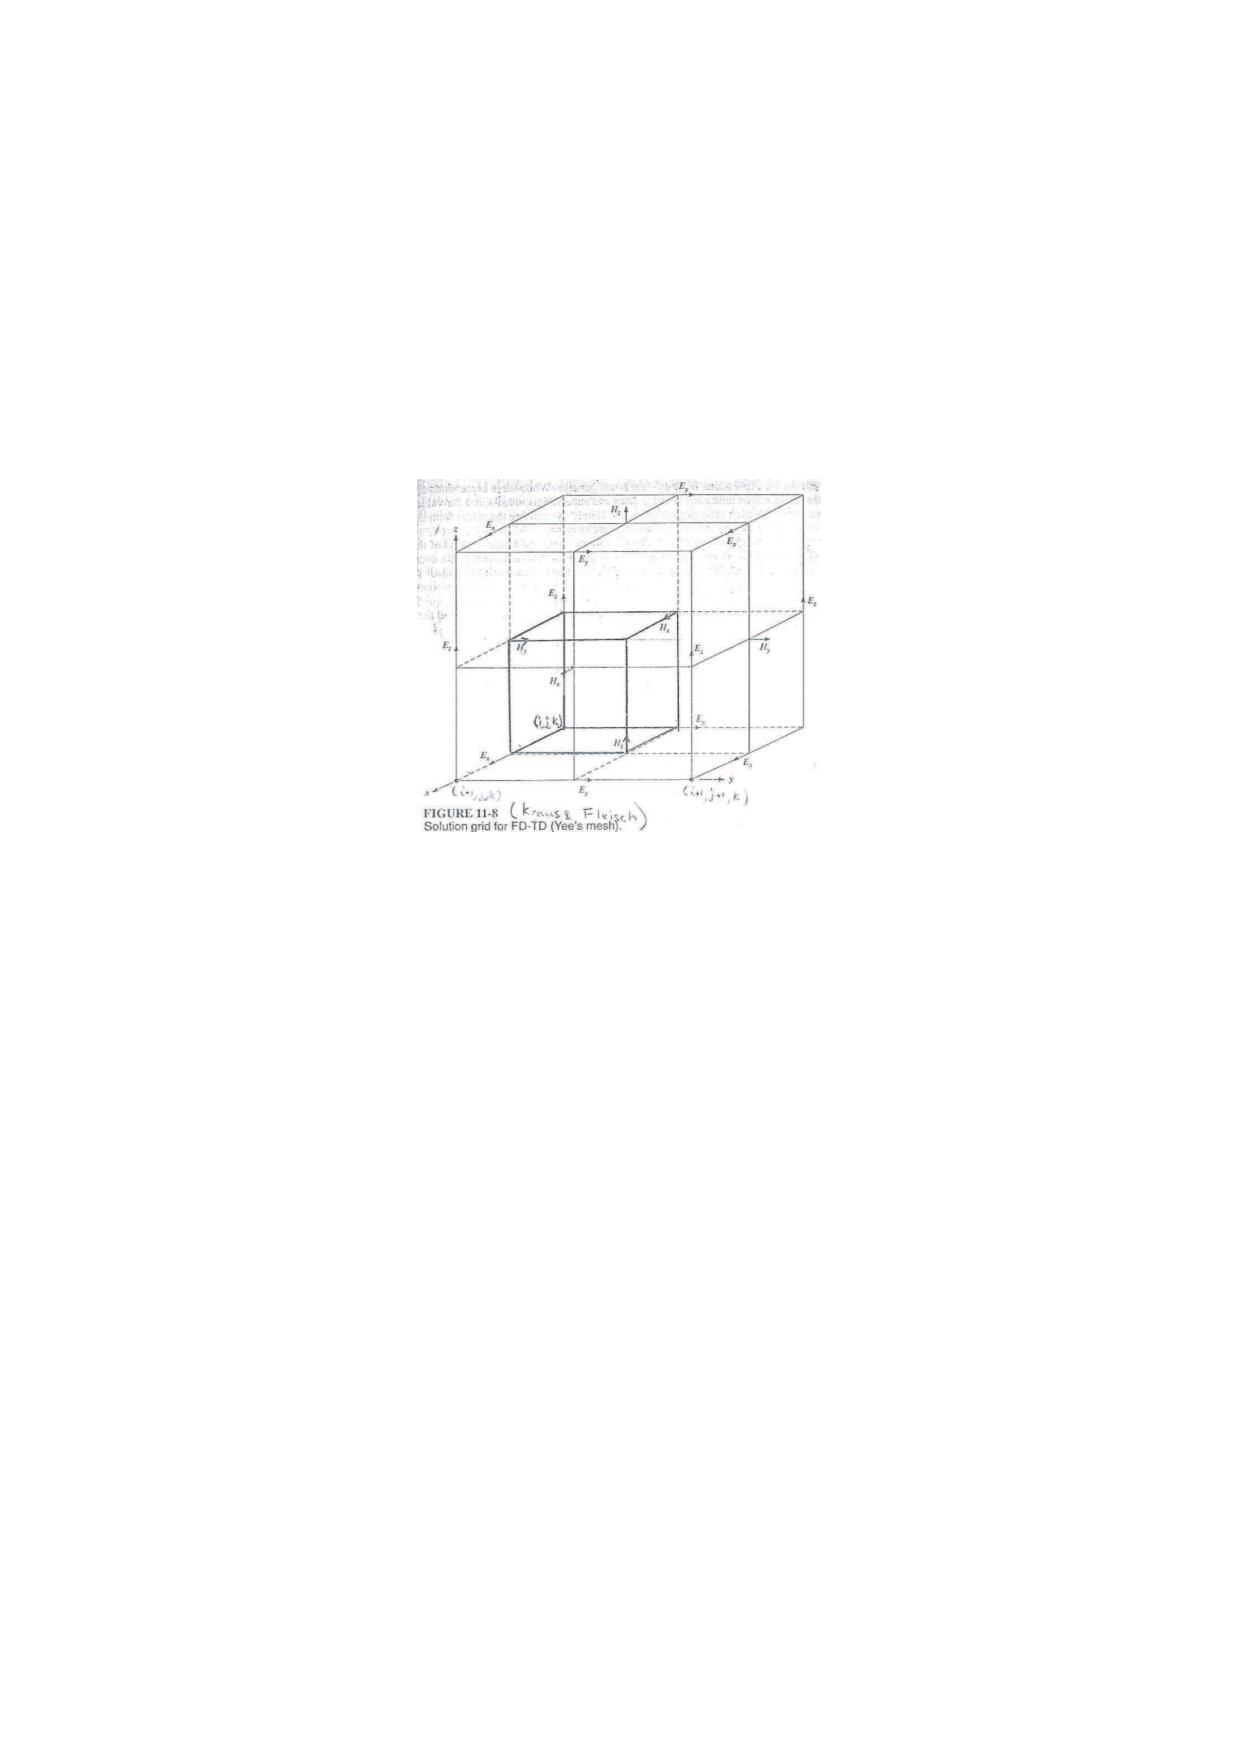
\includegraphics[width=\textwidth]{figures/5.pdf}
		\caption{Diagram illustrating the partitioning of the computational
			space into two regions by the fictitious surface $\Gamma_f$. Only
			the scattered field is calculated in the shaded region whilst the
			total field is calculated in the interior region.}
		\label{fig:numermeth:scat_tot}
	\end{figure}
	The incident
	field is introduced into the total field region by employing an
	additional update equation at the interface between the total and
	scattered regions. This update equation is actually required in order
	to maintain consistency between the scattered and total fields. In
	general, the interface between the total and scattered field is
	a box. Then by applying additional update equations on each face
	of the box, a plane wave of arbitrary propagation direction may be
	introduced to the total field region. This is however much more
	difficult for a more complex incident field such as a focused beam as
	there are so many plane wave components which make up the focused
	beam. The approximate solution to this problem is to introduce an
	interface plane which is extremely wide so that the focused field
	decays to nearly zero at its edges. This implies that the focused
	beam is incident through an aperture but by making the aperture large,
	its effect is made insignificant. Mur \cite{mur81ieeetransemc377} suggested the first kind of absorbing boundary
	condition however a number of other absorbing boundary conditions have
	since been suggested. The PML \cite{berenger94journcopmphys185}, as
	used in the FEM, is now the most widely used absorbing boundary
	condition. As previously explained, it is a layer of absorbing cells
	placed between the scatterer and the PEC boundary of the computational
	grid. The material content of the cells is especially designed such
	that the interface with the homogeneous region has a very low
	reflection.

	A PML must be positioned in between the
	scatterer and the PEC boundary employed around the edge of the
	computational region. The PML was actually developed for use in the
	FDTD method by Berenger \cite{berenger94journcopmphys185} however it
	was not the first absorbing boundary condition to be suggested. Mur
	\cite{mur81ieeetransemc377} suggested the first kind of absorbing boundary
	condition however the PML has been shown to be the best performing
	absorbing boundary condition. The role of the PML is to absorb the the
	scattered field with minimal reflection. Details of how the PML works
	will are given in \sect{sec:fdtd:abcpml}.

	Since FDTD simulations are performed in the time domain, an additional
	step must be performed in order to extract the field in the frequency
	domain. One way of doing this is simply to wait until the fields reach
	a steady state within the computational region. When this method is
	employed, the incident field is introduced gradually and then
	maintained at a constant amplitude until a steady state is
	reached. Once steady state has been reached the time harmonic field
	may be extracted over the course of a few sinusoidal periods. Another
	method that may be employed is to modulate the incident field in time
	by Gaussian pulse but care must be taken to ensure that the pulse is
	sufficiently broad to restrict the bandwidth of the incident
	field. The field at various wavelengths may then be found through
	application of a discrete Fourier transform.

	There are a few restrictions which must be observed in order for the
	FDTD method to work correctly. Firstly, the size of each Yee cell must
	be sufficiently small to accurately sample the field. This is usually
	of the order of $\lambda/20$ or smaller where $\lambda$ is the centre
	wavelength of the incident illumination. There is also an upper bound
	on the time increment used by the method in order to guarantee
	stability of the simulation. In particular, in three dimensions, the
	time increment $\Delta t$ must satisfy the Courant stability criterion \cite{taflove75ieeetransmicrotheoryandtech623}:
	\begin{equation}
		\Delta t \leq \frac{1}{c_{max}}\left(\frac{1}{\Delta x^2} + \frac{1}{\Delta y^2} + \frac{1}{\Delta z^2}\right)^{-1/2}
		\label{eq:numermeth:courant}
	\end{equation}
	where $c_{max}$ is the maximum wave phase velocity expected within
	the model.

	The FDTD method uses memory in linear
	proportion to the number of cells within the computational grid thus
	making it relatively efficient compared with the
	MOM and the Green's tensor method. This however essentially
	implies that it uses memory in linear proportion to the number of
	scattering cells. This means that much larger scatterers can be
	modelled using the FDTD method than can be solved with the MOM and the
	Green's tensor method since as previously explained, these methods use
	memory in proportion with the square of the number of scattering cells.

	\begin{figure}[!h]
		\centering
		%\includegraphics[width=7cm]{fig/yee2.eps}
		\caption{Diagram of a Yee cell \cite{yee66ieeetransantprop302,taflove75ieeetransmicrotheoryandtech623} showing how the various electromagnetic field
			components are sampled.}
		\label{fig:numermeth:yeediag}
	\end{figure}

	The FDTD method has a number of advantages over other methods. The
	first advantage is that it is easy to implement. The simplicity stems
	from the very logical mapping of the algorithm into a computer
	program. Furthermore, the algorithm itself is rather simple. Because
	of the memory efficiency it is
	capable of modelling larger scatterers than the MOM and Green's tensor
	method and at least as big
	as that possible using the FEM. The FDTD method however does not
	suffer from the matrix inversion problem which plagues the FEM. It is
	in fact a very stable method. Another advantage is that the electric
	and magnetic fields are obtained simultaneously with equivalent
	accuracy. A final advantage of the FDTD method is
	that it is a very mature method. It has been applied to numerous
	applications
	\cite{taflove75ieeetransmicrotheoryandtech888,kunz78ieeetransemc328,taflove80ieeetransemc191,sullivan88ieeetransbiomedeng179,joseph91opticsletters31}
	and so a great deal of knowledge has been acquired making the FDTD a
	very powerful tool the electromagnetic scattering calculations.

	The FDTD method does of course have some non ideal attributes. To
	start with, it models dispersive materials poorly. This is because it is necessary to take a frequency domain
	description of a material and convert it to a time domain
	model. Numerous methods have been used (see
	\cite{luebbers90ieeetranseleccomp222} as an example) successfully
	however it must still be considered a weak point of the model. The
	regular orthogonal grid employed by the FDTD method is not suited to
	modelling complex objects. In general, the resolution of object
	features is limited to the grid cell size. Also, curved and sloping
	surfaces must be modelled by a stair case approximation. An example of
	the stair case approximation is shown in
	\rfig{fig:numermeth:staircase}. The diagram shows how a pit used on an
	optical data storage disk is represented with increasingly fine stair
	case approximations. Only the FEM and MOM are able to avoid stair
	casing as they may employ an irregular mesh. Despite these
	disadvantages, the FDTD method is probably the most powerful method
	currently available for performing electromagnetic scattering calculations.
	\begin{figure}[!h]
		\centering
		%\includegraphics[width=7cm]{fig/staircase.eps}
		\caption{Diagram showing the top view of how a optical data storage
			pit is represented using a stair case approximation.}
		\label{fig:numermeth:staircase}
	\end{figure}
	%%%%%
	\section{Implementation details}
	\subsection{Introduction}
	A brief account of the FDTD method is given in
	\sect{sec:numermeth:fdtd}. This chapter contains a more
	comprehensive description of the method. It builds on concepts
	introduced in \sect{sec:numermeth:fdtd} and is intended to be
	largely self supporting.

	\subsection{Discretisation of Maxwell's equations}
	The principle behind the FDTD method is the discretisation in space
	and time of Maxwell's equations in differential
	form. \eqs{eq:numermeth:maxtime1}{eq:numermeth:maxtime2}, repeated
	below for convenience:
	\begin{eqnarray}
		\nabla\times\mathbf{E}&=&-\frac{\partial\mathbf{B}}{\partial t}-\sigma^*\mathbf{H}\nonumber\\
		\nabla\times\mathbf{H}&=&\mathbf{J} + \frac{\partial\mathbf{D}}{\partial t}\nonumber
	\end{eqnarray}
	In conjunction with the constitutive relations
	(\eqs{fig:numermeth:constituted}{fig:numermeth:constituteb}) yield a
	set of coupled partial differential equations of the form:
	\begin{eqnarray}
		\label{eq:fdtd:pdes1}
		\frac{\partial H_x}{\partial t}&=&\frac{1}{\mu_r\mu_0}\left[\frac{\partial E_y}{\partial z}
		-\frac{\partial E_z}{\partial y} - \sigma^*H_x  \right]\\
		\label{eq:fdtd:pdes2}
		\frac{\partial H_y}{\partial t}&=&\frac{1}{\mu_r\mu_0}\left[\frac{\partial E_z}{\partial x}
		-\frac{\partial E_x}{\partial z} - \sigma^*H_y  \right]\\
		\label{eq:fdtd:pdes3}
		\frac{\partial H_z}{\partial t}&=&\frac{1}{\mu_r\mu_0}\left[\frac{\partial E_x}{\partial y}
		-\frac{\partial E_y}{\partial x} - \sigma^*H_z  \right]\\
		\label{eq:fdtd:pdes4}
		\frac{\partial E_x}{\partial t}&=&\frac{1}{\epsilon_r\epsilon_0}\left[\frac{\partial H_z}{\partial y}
		-\frac{\partial H_y}{\partial z} - \left(J_{source_x}+\sigma
		E_x\right)  \right]\\
		\label{eq:fdtd:pdes5}
		\frac{\partial E_y}{\partial t}&=&\frac{1}{\epsilon_r\epsilon_0}\left[\frac{\partial H_x}{\partial z}
		-\frac{\partial H_z}{\partial x} - \left(J_{source_y}+\sigma
		E_y\right)  \right]\\
		\label{eq:fdtd:pdes6}
		\frac{\partial E_z}{\partial t}&=&\frac{1}{\epsilon_r\epsilon_0}\left[\frac{\partial H_y}{\partial x}
		-\frac{\partial H_x}{\partial y} - \left(J_{source_z}+\sigma E_z\right)  \right]
	\end{eqnarray}
	where the substitution $\mathbf{J} = \mathbf{J}_{source} +
	\sigma\mathbf{E}$ has been made in order to represent both conduction
	currents ($\sigma\mathbf{E}$) and current sources
	($\mathbf{J}_{source}$) within the
	computational domain. In order
	to proceed, the computational volume must be partitioned into a number
	of cuboid cells as demonstrated in \rfig{fig:fdtd:fdtdgrid}. Each
	field component is sampled once per cuboid cell in the manner
	suggested by Yee \cite{yee66ieeetransantprop302} and is shown in \rfig{fig:numermeth:yeediag}. Thus each cuboid
	shown in \rfig{fig:fdtd:fdtdgrid} contains a Yee cell. The position of field
	sample points within the computational volume is described by a set of
	indices $(i,j,k)$ which correspond to position
	$(i\Delta_x,j\Delta_y,k\Delta_z)$ where $\Delta_x$, $\Delta_y$ and
	$\Delta_z$ are the lengths of the Yee cell in the $x$-, $y$- and $z$-directions respectively. Thus the computational volume may be gridded
	with different resolution in each of the three orthogonal directions.


	The arrangement of the Yee cell is important for two primary reasons. Firstly, it is ideal for imposing PEC boundary conditions
	on any face of the cell. This is because each face of the Yee cell
	contains components of electric field tangential to the face and a
	component of the magnetic field normal to the face. Thus a PEC
	boundary can be set on any face simply by setting these values to 0. Secondly, the
	field components are positioned such that central differences (see
	\sect{sec:numermeth:fdtd}) between
	components may be evaluated where they are required. For example,
	\eq{eq:fdtd:pdes1} involves the terms $\frac{\partial E_y}{\partial
		z}$ and $\frac{\partial E_z}{\partial y}$. Using
	\eq{eq:numermeth:centdiff} it becomes clear that in order to
	approximate these derivatives at a particular point in space using
	central differences, this
	point must be positioned in the middle of a line parallel to the
	$z$-axis joining two $E_y$ sample points and on the middle of a line
	parallel to the $y$-axis joining two $E_z$ sample points. This is
	precisely where the $H_x$ sample point is located in the Yee cell,
	demonstrating why the Yee cell is arranged in the way that it is.
	\begin{figure}[!h]
		\centering
		%\includegraphics[width=7cm]{fdtd/fig/grid/fdtdgrid.eps}
		\caption{Gridding of computational volume into cuboid cells. A stair
			case approximation of a scatterer is indicated by the shaded cells.}
		\label{fig:fdtd:fdtdgrid}
	\end{figure}

	Time must also be sampled. This is done by selecting a time step
	$\Delta t$ which describes the spacing in time of successive samples in
	the simulation. In order to facilitate central differences in time,
	the magnetic and electric fields are calculated half a time step
	apart. Time within the simulation is denoted by an index $n$ which
	corresponds to time $n\Delta t$. Using this system of indexing space
	and time, field components are indexed as, for example,
	$E_x|^{n+1/2}_{i,j+1/2,k+1/2}$ which denotes the value of $E_x$ at
	time $t=(n+1/2)\Delta t$ and position $(i\Delta_x,(j+1/2)\Delta_y,
	(k+1/2)\Delta_z)$. The diagram in \rfig{fig:fdtd:tfsfeg} shows that
	if the Yee cell is centred on position $(i,j,k)$ then the $E_x$
	component is indeed located at $(i,j+1/2,k+1/2)$.

	By employing this sampling scheme in space and time and approximating
	each derivative in \eqr{eq:fdtd:pdes1}{eq:fdtd:pdes6} with a central difference
	operation (see \sect{sec:numermeth:fdtd}), the following set of
	difference equations is obtained after some manipulations \cite{taflove00book}:
	\begin{align}
		\label{eq:fdtd:diff1}
		E_x|^{n+1/2}_{i,j+1/2,k+1/2}=&C_a|_{i,j+1/2,k+1/2}E_x|^{n-1/2}_{i,j+1/2,k+1/2}+\nonumber\\
		& C_{b_y}|_{i,j+1/2,k+1/2}\left(H_z|^n_{i,j+1,k+1/2} -
		H_z|^n_{i,j,k+1/2}\right)+\nonumber\\&C_{b_z}|_{i,j+1/2,k+1/2}\left(H_y|^n_{i,j+1/2,k}-H_y|^n_{i,j+1/2,k+1}\right)-\nonumber\\&C_{b_x}|_{i,j+1/2,k+1/2}{J_{source_x}}|^n_{i,j+1/2,k+1/2}\Delta_x
		\\
		\label{eq:fdtd:diff2}
		E_y|^{n+1/2}_{i-1/2,j+1,k+1/2}=&C_a|_{i-1/2,j+1,k+1/2}E_y|^{n-1/2}_{i-1/2,j+1,k+1/2}+\nonumber\\
		&C_{b_z}|_{i-1/2,j+1,k+1/2}\left(H_x|^n_{i-1/2,j+1,k+1} -
		H_x|^n_{i-1/2,j+1,k}\right)+\nonumber\\&C_{b_x}|_{i-1/2,j+1,k+1/2}\left(H_z|^n_{i-1,j+1,k+1/2}-H_z|^n_{i,j+1,k+1/2}\right)-\nonumber\\&C_{b_y}|_{i-1/2,j+1,k+1/2}{J_{source_y}}|^n_{i-1/2,j+1,k+1/2}\Delta_y\\
		\label{eq:fdtd:diff3}
		E_z|^{n+1/2}_{i-1/2,j+1/2,k+1}=&C_a|_{i-1/2,j+1/2,k+1}E_z|^{n-1/2}_{i-1/2,j+1/2,k+1}+\nonumber\\
		&C_{b_x}|_{i-1/2,j+1/2,k+1}\left(H_y|^n_{i,j+1/2,k+1} -
		H_y|^n_{i-1,j+1/2,k+1}\right)+\nonumber\\&C_{b_y}|_{i-1/2,j+1/2,k+1}\left(H_x|^n_{i-1/2,j,k+1}-H_x|^n_{i-1/2,j+1,k+1}\right)-\nonumber\\&C_{b_z}|_{i-1/2,j+1/2,k+1}{J_{source_z}}|^n_{i-1/2,j+1/2,k+1}\Delta_z\\
		\label{eq:fdtd:diff4}
		H_x|^{n+1}_{i-1/2,j+1,k+1}=&D_a|_{i-1/2,j+1,k+1}H_x|^{n}_{i-1/2,j+1,k+1}+\nonumber\\
		& D_{b_z}|_{i-1/2,j+1,k+1}\left(E_y|^{n+1/2}_{i-1/2,j+1,k+3/2} -
		E_y|^{n+1/2}_{i-1/2,j+1,k+1/2}\right)+\nonumber\\&D_{b_y}|_{i-1/2,j+1,k+1}\left(E_z|^{n+1/2}_{i-1/2,j+1/2,k+1}-E_z|^{n+1/2}_{i-1/2,j+3/2,k+1}\right)\\
		\label{eq:fdtd:diff5}
		H_y|^{n+1}_{i,j+1/2,k+1}=&D_a|_{i,j+1/2,k+1}H_y|^{n}_{i,j+1/2,k+1}+\nonumber\\
		&D_{b_x}|_{i,j+1/2,k+1}\left(E_z|^{n+1/2}_{i+1/2,j+1/2,k+1} -
		E_z|^{n+1/2}_{i-1/2,j+1/2,k+1}\right)+\nonumber\\&D_{b_z}|_{i,j+1/2,k+1}\left(E_x|^{n+1/2}_{i,j+1/2,k+1/2}-E_x|^{n+1/2}_{i,j+1/2,k+3/2}\right)\\
		\label{eq:fdtd:diff6}
		H_z|^{n+1}_{i,j+1,k+1/2}=&D_a|_{i,j+1,k+1/2}H_z|^{n}_{i,j+1,k+1/2}+\nonumber\\
		&D_{b_y}|_{i,j+1,k+1/2}\left(E_x|^{n+1/2}_{i,j+3/2,k+1/2} -
		E_x|^{n+1/2}_{i,j+1/2,k+1/2}\right)+\nonumber\\&D_{b_x}|_{i,j+1,k+1/2}\left(E_y|^{n+1/2}_{i-1/2,j+1,k+1/2}-E_y|^{n+1/2}_{i+1/2,j+1,k+1/2}\right)
	\end{align}
	where
	\begin{eqnarray}
		\label{eq:fdtd:ca}
		C_{a}|_{i,j,k}&=&\left(1-\frac{\sigma_{i,j,k}\Delta
			t}{2\epsilon_{r_{i,j,k}}\epsilon_0}\right)/\left(1+\frac{\sigma_{i,j,k}\Delta
			t}{2\epsilon_{r_{i,j,k}}\epsilon_0}\right)\\
		\label{eq:fdtd:cb}
		C_{b_s}|_{i,j,k}&=&\left(\frac{\Delta t}{\epsilon_{r_{i,j,k}}\epsilon_0\Delta_s}\right)/\left(1+\frac{\sigma_{i,j,k}\Delta
			t}{2\epsilon_{r_{i,j,k}}\epsilon_0}\right)\\
		\label{eq:fdtd:da}
		D_{a}|_{i,j,k}&=&\left(1-\frac{\sigma^*_{i,j,k}\Delta
			t}{2\mu_{r_{i,j,k}}\mu_0}\right)/\left(1+\frac{\sigma^*_{i,j,k}\Delta
			t}{2\mu_{r_{i,j,k}}\mu_0}\right)\\
		\label{eq:fdtd:db}
		D_{b_s}|_{i,j,k}&=&\left(\frac{\Delta t}{\mu_{r_{i,j,k}}\mu_0\Delta_s}\right)/\left(1+\frac{\sigma^*_{i,j,k}\Delta
			t}{2\mu_{r_{i,j,k}}\mu_0}\right)
	\end{eqnarray}
	and $\sigma_{i,j,k}$, $\sigma^*_{i,j,k}$, $\epsilon_{r_{i,j,k}}$ and
	$\mu_{r_{i,j,k}}$ are the conductivity, equivalent magnetic loss,
	relative permittivity and relative permeability respectively at grid
	location $(i,j,k)$. $s$ can be either of the orthogonal Cartesian axes
	labels $x$, $y$ or $z$. Scatterers may thus be built up by specifying a
	distribution of the above parameters which depends upon grid position
	$(i,j,k)$. Note that it is also necessary to make the so called
	semi-implicit approximation: $E_s|^n=(E_s|^{n+1/2}+E_s^{n-1/2})/2$ in
	order to treat the magnetic loss and conductivity terms appearing in \eqr{eq:fdtd:pdes1}{eq:fdtd:pdes6}.

	This system of difference equations provides a means by which, given
	$\mathbf{E}|^{n-1/2}$ and $\mathbf{H}|^n$ throughout the computational
	grid, $\mathbf{E}|^{n+1/2}$ may be
	found which may in turn be used, together with $\mathbf{H}|^n$ to
	calculate $\mathbf{H}|^{n+1}$. Thus, given an initial electromagnetic
	field throughout the entire computational volume, the electromagnetic
	field may be found at any later time subject to the time sampling
	scheme employed in the simulation. Note that this assumes the use of a
	boundary condition at the boundary of the computational region. This
	is dealt with in \sect{sec:fdtd:abcpml}.

	\subsection{Introducing an incident waveform}
	\label{sec:fdtd:incwave}
	Scattering problems typically have
	an incident illumination which gives rise to a scattered field. The
	method most commonly employed to introduce an incident wave into a
	simulation is called the Total Field/Scattered Field (TF/SF)
	formulation
	\cite{mur81ieeetransemc377,umashankar82ieeetransemc397}. This method
	works by partitioning the computational region into two volumes as
	shown in \rfig{fig:fdtd:tfsf}. The linearity of Maxwell's equations
	permits the total electromagnetic field to be decomposed as:
	\begin{equation}
		(\mathbf{E},\mathbf{H}) = (\mathbf{E}^i,\mathbf{H}^i) + (\mathbf{E}^s,\mathbf{H}^s)\nonumber
	\end{equation}
	where $(\mathbf{E}^i,\mathbf{H}^i)$ is the field due solely to the
	incident field in the absence of a scatterer and is generally known
	analytically. The scattered field $(\mathbf{E}^s,\mathbf{H}^s)$ is the
	difference between the total field actually present and the incident
	field. $(\mathbf{E}^i,\mathbf{H}^i)$ and $(\mathbf{E},\mathbf{H})$
	must satisfy Maxwell's equations in the homogeneous space surrounding
	the scatterer and as a result so must
	$(\mathbf{E}^s,\mathbf{H}^s)$. Inside the scatterer,
	$(\mathbf{E}^s,\mathbf{H}^s)$ should be considered the perturbation to
	the incident field to ensure that the total field satisfies Maxwell's
	equations. It should be stressed that this
	representation is not an approximation, simply a convenient
	decomposition of the field.
	\begin{figure}[!h]
		\centering
		%\includegraphics[width=7cm]{fdtd/fig/tfsf.eps}
		\caption{Diagram showing the partitioning the computational volume
			into total field and scattered field regions separated by the
			fictitious surface $\Gamma_f$.}
		\label{fig:fdtd:tfsf}
	\end{figure}
	To demonstrate how the incident waveform is introduced consider the
	example depicted in \rfig{fig:fdtd:tfsfeg}. The shaded plane through
	the Yee cell centre marks the boundary between the scattered and total
	field regions. The scattered field is stored for values of $y$ less than
	where the boundary is positioned and the total field is stored
	elsewhere. Consider the update equation for H$_{z,1}$, given by
	\eq{eq:fdtd:diff6}. It is incorrect to apply this equation, without
	modification, to update H$_{z,1}$ as the update equation would contain
	terms which are from the scattered field region and some which are
	from the total field region. The incident field is however generally
	known analytically and so the update equation for H$_{z,1}$ may be
	written as:
	\begin{eqnarray}
		H_{z,1}|^{n+1}&=& D_aH_{z,1}|^n+D_b\left(E_{x,2}|^{n+1/2} -
		\left(E_{x,1}^s|^{n+1/2}+E_{x,1}^i|^{n+1/2}\right) + \nonumber\right.\\&&\left.E_{y,1}|^{n+1/2}
		- E_{y,2}|^{n+1/2}\right)\nonumber\\
		&=&D_a H_{z,1}|^n+D_b\left(E_{x,2}|^{n+1/2} -
		E_{x,1}^s|^{n+1/2} + E_{y,1}|^{n+1/2}
		- E_{y,2}|^{n+1/2}\right)-\nonumber\\&&D_bE^i_{x,1}|^n\label{eq:fdtd:tfsfupdate}
	\end{eqnarray}
	where it has been assumed that $\Delta_x=\Delta_y=\Delta$ and thus
	$D_{b_x}=D_{b_y}$. \eq{eq:fdtd:tfsfupdate} implies that the FDTD algorithm may proceed as normal across the
	interface but an additional term, $D_bE^i_{x,1}|^n$, must be
	subtracted from the standard update equation in order to maintain
	consistency between the total and scattered regions. Similar equations
	for each update equation arise at each part of the cuboid boundary
	between the scattered and total fields. These may be viewed in Taflove
	and Hagness \cite{taflove00book}.
	\begin{figure}[!h]
		\centering
		%\includegraphics[width=7cm]{fdtd/fig/PM_Yee_1.eps}
		\caption{Diagram showing the boundary between scattered and total
			field regions and a Yee cell.}
		\label{fig:fdtd:tfsfeg}
	\end{figure}

	The temporal properties of the waveform to be introduced must be
	considered very carefully. For instance, if the time harmonic field of
	an incident wave is known then it could be introduced simply by
	``switching on'' the source at a particular time as if the source was
	modulated by a step function. This would however introduce high
	frequency components into the incident waveform which would degrade
	the accuracy of the simulation as the FDTD grid resolution is chosen
	so as to sample all spectral components adequately. This problem may
	be solved by gradually and smoothly increasing the amplitude of the
	incident waveform from 0 till the required amplitude is reached. This
	limits the introduction of high frequency components. The simulation is then
	allowed to proceed until a steady state is reached. The simulation
	must determine when steady state has been reached by comparing the
	field within the computational region over successive sinusoidal
	cycles. Extraction of the complex amplitude of the field phasors allow
	the time harmonic field to be extracted from the simulation.

	An alternative to this method is to introduce an incident wave
	modulated by a single Gaussian pulse. The Gaussian pulse provides a
	way to accurately control the spectral width of the incident field. The time harmonic scattered field may then be found from the time
	domain scattered field by application of a Discrete Fourier Transform
	(DFT). When this method is used, the incident field in the time domain is
	given by:
	%\begin{equation}
	%\label{eq:fdtd:tdinc}
	%\mathbf{E}^{inc}(\mathbf{r},t)=\Re\left\{-\imath\mathbf{E}_0^{inc}(\mathbf{r})\exp(-\imath\omega_0(t-t_0))\exp\left(-\pi\left(\frac{t-t_0}{W_0}\right)^2\right)\right\}
	%\end{equation}
	\begin{equation}
		\label{eq:fdtd:tdinc}
		\mathbf{E}^{inc}(\mathbf{r},t)=\Re\left\{\imath\mathbf{E}_0\exp(\imath(k_0\boldsymbol{\beta}\!\cdot\!\mathbf{r}-\omega_0(t-t_0)))\exp\left(-\pi\left(\frac{t-(t_0+\boldsymbol{\beta}\!\cdot\!\mathbf{r}/c)}{W_0}\right)^2\right)\right\}
	\end{equation}
	where $\Re$ denotes the real part, $\mathbf{E}_0$ is the
	polarisation of the plane wave,
	$\omega_0$ and $k_0$ are the angular frequency and wavenumber of the
	wave in the homogeneous region, $\boldsymbol{\beta}$ is the unit vector in the
	direction of propagation of the plane wave, $W_0$
	controls the pulse width, $t_0$ controls the delay of the pulse
	peak, $c$ is the speed of light in the homogeneous region and $\mathbf{r}$ is the position within the computational volume. Note that the factor of $\imath$ appears to ensure that the
	pulse has 0 DC content. $W_0$
	must be chosen so that the spectral width of the incident waveform is
	sufficiently narrow and $t_0$ is chosen to ensure that the incident
	waveform starts with a vanishingly small amplitude. In particular, the
	spectral width of the modulating pulse may be analysed by taking the
	Fourier transform of $\exp(-\pi(t/W_0)^2)$ as:
	\begin{equation}
		\label{eq:fdtd:specwid}
		\mathfrak{F}\left\{\exp(-\pi(t/W_0)^2)\right\}=W_0\exp(-\pi(fW_0)^2)
	\end{equation}
	where $\mathfrak{F}$ is the Fourier transform operator. Then the
	spectral width of the incident waveform, $\Delta f$, defined as the
	Full Width at Half Maximum (FWHM) of $W_0\exp(-\pi(fW_0)^2)$ is given
	by $\Delta f=2/W_0\sqrt{\log 2/\pi}$. The wavelength width is however
	of more interest, which may be found using the relationships
	$f\lambda=c$ and $\Delta f\approx -c/\lambda^2\Delta \lambda$ as
	$\Delta \lambda=2\lambda^2/(c W_0)\sqrt{\log 2/\pi}$. Thus $W_0$ may
	be chosen to guarantee a particular $\Delta \lambda$. It is shown in a
	later section that a sufficient value of $\Delta \lambda/\lambda$ is
	of the order of 0.1. $t_0$ is set so that when the source starts at $t=0$,
	it has a very small amplitude. Testing shows that an initial
	magnitude of 8 orders of magnitude below the peak amplitude is
	sufficient.

	The time domain expression of the incident field, \eq{eq:fdtd:tdinc}, is discretised as
	required by the FDTD update equations which maintain the consistency
	between scattered and total field regions. At each time step the
	incident field update equations are executed. The simulation must be
	run until the scattered field has decayed to many orders of magnitude
	lower than the peak scattered field. The time harmonic
	scattered field may then be found by application of a DFT to the time
	domain scattered field data. This may be done efficiently by
	considering the DFT of an arbitrary function $g(t)$ which may be
	considered as one of the field components. Then the DFT $G(f_0)$ is evaluated
	according to:
	\begin{equation}
		\label{eq:fdtd:dft}
		G(f_0)=\frac{1}{N}\sum^{N-1}_{k=0}g(k\Delta t)\exp(\imath2\pi f_0 k\Delta t)
	\end{equation}
	where $N$ is the number of times $g(t)$ is sampled, $\Delta t$ is the
	time between sample points and $f_0$ is the frequency at which the DFT
	is evaluated. Since the FDTD simulation steps through each of the
	indices $k=0$ to $N-1$, this sum is best evaluated incrementally as
	the simulation progresses. This avoids the need to store the complete
	time evolution of the scattered field which would be unfeasible. This
	is not the end of the story as the frequency spectrum of the incident
	field must be taken into account. This is most conveniently done by
	calculating the DFT of the modulating pulse concurrently with the
	field DFT. The time harmonic scattered field at a particular frequency
	may then be found by dividing the DFT of the field by the DFT of the
	modulating pulse at the frequency of interest.

	This method of introducing an incident field using a pulsed excitation
	is preferred since it avoids the problem of establishing when the
	field reaches a steady state. Also, as an added bonus, it allows the
	broadband response of a structure to be calculated based upon a single
	FDTD simulation.

	The incident wave theory represented hitherto is valid only for a single
	plane wave excitation. This is because a particular direction of
	propagation of the wave front must be chosen in order that the
	amplitude of the modulating pulse may be calculated at the boundary
	between the total and scattered field regions. Thus one way of
	modelling a complex incident waveform is to decompose it into an
	angular spectrum representation. An FDTD simulation would then need to
	be carried out for each plane wave component or multiple update
	equations would need to be applied at the boundary between total and
	scattered field, one for each plane wave component. Both of these
	methods are computationally demanding. Fortunately there is an
	approximation which may be used in the case where the incident wave is
	a focused beam.

	In the vicinity of the focus of a high NA lens, the field decays
	extremely quickly in the transverse direction. Thus it is possible to
	define a window transverse to the optical axis of the lens, positioned
	near the focus of the lens such that most of the energy of the beam
	propagates through the window. Thus the field at the edges of the
	window are vanishingly small. When this is the case it is possible to
	neglect the update equations on the edges of the window. This allows a
	complex waveform to be launched into the computational volume with
	minimum computational load.

	This approximation may be interpreted in a number of ways. Firstly it
	may be considered that the focused beam is apertured. Since the aperture is large compared to the focused spot
	it has a negligible effect. Secondly, this is very similar to the way
	waveguides are modelled using the FDTD method. If the field were being launched into a
	waveguide it would be completely valid. The validity of this
	approximation will be considered in \sect{sec:fdtd:focuselight}.
	\subsection{Numerical dispersion}
	\label{sec:fdtd:numdisp}
	Ideally, the phase velocity of a plane wave propagating within a
	homogeneous FDTD computational volume is determined entirely by the
	material properties of the computational volume. This is not the
	case. The FDTD method introduces what is known as numerical dispersion
	into the obtained solution. This arises because the grid size and time
	step place a constraint on the phase velocity of waves travelling in
	the FDTD system. A full analysis of numerical dispersion is beyond the
	scope of this section however it is possible to obtain some results
	for restricted cases.

	The strategy is as outlined by Taflove \cite{taflove00book} and
	involves postulating a trial solution for a plane wave propagating
	within a FDTD simulation. The solution obtained at an arbitrary time
	step using the FDTD method is equated with the analytic solution of
	the wave being launched into the system. The resulting system of
	equations permits the relationship between phase velocity, grid size
	and time step to be established. The relationship given by Taflove
	\cite{taflove00book} for a plane wave propagating in a three
	dimensional Yee grid is:
	\begin{eqnarray}
		\left[\frac{1}{c\Delta t}\sin\left(\frac{\omega\Delta
			t}{2}\right)\right]^2 &=& \left[\frac{1}{\Delta_x}\sin\left(\frac{\tilde{k}_x\Delta_x}{2}\right)\right]^2+\left[\frac{1}{\Delta_y}\sin\left(\frac{\tilde{k}_y\Delta_y}{2}\right)\right]^2+\nonumber\\&&\left[\frac{1}{\Delta_z}\sin\left(\frac{\tilde{k}_z\Delta_z}{2}\right)\right]^2
		\label{eq:fdtd:numdisp1}
	\end{eqnarray}
	where $\omega$ is the angular frequency of the numerical wave and
	$\tilde{k}=(\tilde{k}_x,\tilde{k}_y,\tilde{k}_z)$ is the wave vector
	of the numerical wave. This relationship is too complex to analyse in
	three dimensions and so the problem is reduced to two dimensions by
	selecting $k_z=0$. Then a numerical wave propagating at an angle
	$\phi$ to the $x$-axis of the numerical grid with
	$\Delta=\Delta_x=\Delta_y$ is postulated. This
	results in the following dispersion relation:
	\begin{eqnarray}
		\frac{1}{S^2}\sin^2\left(\frac{\pi
			S}{N_\lambda}\right)=\sin^2\left(\frac{\Delta\tilde{k}\cos\phi}{2}\right)
		+ \sin^2\left(\frac{\Delta \tilde{k}\sin\phi}{2}\right)
		\label{eq:fdtd:numdisp2}
	\end{eqnarray}
	where $S$ is the Courant number defined as $S=c\Delta t/\Delta$ and
	$N_\lambda$ is the grid sampling density defined as
	$N_\lambda=\lambda_0/\Delta$ where $\lambda_0$ is the wavelength of
	the numerical wave. The objective is to solve for $\tilde{k}$ given
	$S$, $N_\lambda$, $\Delta$ and $\phi$. This cannot be done easily in
	general and a numerical method, such as Newton's method as suggested
	by Taflove \cite{taflove00book}, must be employed. Using this method,
	a plot (see \rfig{fig:fdtd:numdispphi}) of normalised phase velocity $v_p/c$ for a numerical wave
	propagating in a vacuum has been calculated a function of propagation
	angle $\phi$. The plot corresponds to the case $S=0.5$ and
	$N_\lambda=20$.
	\begin{figure}[!h]
		\centering
		%\includegraphics[width=7cm]{fdtd/sims/numdispphi.eps}
		\caption{Plot of normalised phase velocity as a function of
			propagation angle within the FDTD grid. Corresponds to the case
			$S=0.5$ and $N_\lambda=20$.}
		\label{fig:fdtd:numdispphi}
	\end{figure}
	This plot illustrates the general relationship between propagation
	angle and normalised phase velocity. Numerical dispersion may be
	reduced by increasing $N_\lambda$. \rfig{fig:fdtd:numdispN} shows a
	plot of $1-v_p/c$ for a numerical wave with $\phi=\pi/4$, $S=0.5$ and
	increasing values of $N_\lambda$. The plot demonstrates that even at
	what is considered an impractical value for $N_\lambda$, there is
	still numerical dispersion.
	\begin{figure}[!h]
		\centering
		%\includegraphics[width=7cm]{fdtd/sims/numdispN.eps}
		\caption{Plot showing 1-$v_p/c$ as a function of
			$N_\lambda$. Corresponds to case of $S=0.5$ and $\phi=\pi/4$.}
		\label{fig:fdtd:numdispN}
	\end{figure}
	\subsection{Numerical stability}
	The FDTD method is not unconditionally numerically stable. The time
	step must be bounded in order to maintain stability. Taflove
	\cite{taflove00book} shows that the following relationship must hold
	in order for the scheme to remain numerically stable:
	\begin{equation}
		\label{eq:fdtd:stab}
		0\le c\Delta t\sqrt{\frac{1}{\Delta^2_x}+\frac{1}{\Delta^2_y}+\frac{1}{\Delta^2_z}}\le1
	\end{equation}
	where $c$ is the speed of light in the fastest region of the
	computational space. In the special case of a cubic grid in three
	dimensions this reduces down to the simple case:
	\begin{equation}
		\Delta t\le\frac{\Delta}{c\sqrt{3}}
		\label{eq:fdtd:stabsimp}
	\end{equation}
	\subsection{Selection of grid resolution}
	The size of the Yee cell must be selected carefully to ensure the
	simulation is sufficiently accurate. Recall from
	\sect{sec:numermeth:fdtd} that central difference operations have an
	error of the order of the square of the distance between sample
	points. Thus supposing that $\Delta$ is the maximum of $\Delta_x$,
	$\Delta_y$ and $\Delta_z$, the error associated with each difference
	operation would be $O(\Delta^2)$. By looking at the derivation of this
	result it becomes evident that the central difference operation
	produces an exact result for quantities which vary linearly. Thus
	$\Delta$ should be chosen sufficiently small such that the waveforms
	vary approximately linearly between field component sample points on
	adjacent Yee cells. As a general rule, $\Delta$ is chosen to be no larger than
	$\lambda/20$.

	Accuracy is however not the only factor which affects the choice of
	$\Delta$. This is because all scattering objects must be built up
	using a staircase approximation. Thus, small features must be
	constructed using cuboids with sides of at least $\Delta$ in
	length. Thus the choice of $\Delta$ is determined not only by the need
	to accurately sample the field but also to accurately model the scatterer.
	\subsection{Absorbing boundary conditions}
	\label{sec:fdtd:abcpml}
	Scattering problems in
	optics generally involve a scatterer in an infinite space or infinite
	half space. Due to computers having only a finite amount of memory,
	the computational region must be truncated somehow using an approximate
	boundary condition which closely approximates an infinite boundary
	condition. It is very difficult to devise such a boundary
	condition based solely upon Maxwell's equations in a difference method
	such as the FDTD method. This is because at the boundary of the
	computational space, not all difference operations can be evaluated
	because some data is missing, in particular those data points which
	would be outside the artificial boundary of the computational
	domain. A boundary condition of this type is called an Absorbing Boundary Condition (ABC).

	ABCs result in a boundary condition with an extremely low reflection
	of outgoing radiation. An ideal ABC would absorb all outgoing
	radiation without reflecting any back into the computational
	volume. In practice there is always a small reflection however as long
	as the reflection is sufficiently small the ABC will not be the factor
	limiting the simulation accuracy.

	The first generations of absorbing boundary conditions were all what
	are known as analytic ABCs. These have largely been made redundant due
	to the development of the Perfectly Matched Layer (PML) which will be
	discussed later in this section. Analytic ABCs either try to calculate
	the difference operations which cannot be evaluated due to missing
	data at the computational space boundary or use an alternative
	difference scheme at the boundary. For example, radiation operators
	\cite{bayliss82siamjappmath430,bayliss80commpapplmath707,higdon87mathcomp65,higdon86mathcomp437}
	provide a means for estimating the derivative of a propagating wave in
	the direction of propagation based upon spatial derivatives transverse
	to the direction of propagation and temporal derivatives. This
	provides a way to approximate the derivatives which otherwise could not
	be calculated because of missing data. Another class of analytic ABCs
	use what is known as a one-way wave equation
	\cite{engquist77mathcomp629,mur81ieeetransemc377,trefethen86mathcomp421}
	to devise an alternative differencing scheme to be applied at the
	boundary of the computational region. A one-way wave equation is a wave equation which permits
	propagation of a wave in one direction only. The final class of analytic
	ABCs uses a scheme to extrapolate from historical data the field at
	the missing data points \cite{taflove00book}. This draws upon the principle of retarded
	radiation so that data
	from an earlier time is used to calculate the field at a later time at
	points located further from the scatterer than the initial points. These
	methods have been used to good effect over a period of decades. The
	PML has now superseded them in most applications. The theory behind
	the PML will be discussed now.

	The previously introduced analytic ABCs all use different update
	equations on the boundary of the computational space. The PML operates
	in quite a different manner. A PML is a layer of absorbing material
	placed between the scatterer and a PEC boundary which terminates the
	computational space. The material is designed such that it has, in
	principle, zero reflection for plane waves of any frequency
	propagating at arbitrary angle of incidence relative to the PML
	boundary. The absorbing nature of the PML causes waves which
	propagate through it to be attenuated such that there is very little energy reflected
	back of the PEC boundary. As long as the PML is situated in the
	scattered field region of the FDTD computational space it is very
	useful for simulating open region scattering problems.

	The PML was first introduced in two dimensions by Berenger
	\cite{berenger94journcopmphys185} and then later in three dimensions
	\cite{berenger96journalcopmphys363}. Berenger's formulation employs a
	non-physical modification of Maxwell's equations. For brevity a full
	derivation of Berenger's PML will not be presented but the salient
	details will be. To understand how such a material may be constructed,
	consider a plane wave incident normally upon an interface between two
	materials as shown in \rfig{fig:fdtd:fresnel}. Using Fresnel's
	equations it may be shown that to eliminate the reflected wave
	($\mathbf{E}_r$ and $\mathbf{H}_r$), the following relationship must
	hold:
	\begin{equation}
		\label{eq:fdtd:zeroref}
		\mu^*_1k_0n_2=\mu_2^*k_0n_1
	\end{equation}
	where $k_0$ is the wave number in material 1, $\mu_1^*=\mu_{r1}\mu_0$,
	$\mu^*_2=\mu_{r1}\mu_0(1-\sigma_2^*/\imath\omega_0\mu_{r2}\mu_0)$,
	$n_2=\sqrt{\mu_2^*\epsilon_2^*}/\sqrt{\epsilon_0\mu_0}$,
	$n_1=\sqrt{\mu_1^*\epsilon_1^*}/\sqrt{\epsilon_0\mu_0}$,
	$\epsilon_2^*=\epsilon_{r2}\epsilon_0(1-\sigma_2/(\imath\omega_0\epsilon_{r2}\epsilon_0)$,
	$\epsilon^*_1=\epsilon_{r1}\epsilon_0$ and $\omega_0$ is the angular
	frequency of the time harmonic plane wave.
	\begin{figure}[!h]
		\centering
		%\includegraphics[width=7cm]{fdtd/fig/fresnel.eps}
		\caption{Figure showing a plane wave normally incident upon an
			interface between a dielectric and a conducting material.}
		\label{fig:fdtd:fresnel}
	\end{figure}
	Some manipulations show that \eq{eq:fdtd:zeroref} requires that
	$\sqrt{\epsilon_1^*/\mu_1^*}=\sqrt{\epsilon_2^*/\mu_2^*}$. This in
	turn requires that $\epsilon_{r2}/\epsilon_{r1}=\mu_{r2}/\mu_{r1}$ and
	$\sigma_2^*/\mu_{r1}=\sigma_2/\epsilon_{r1}$. This provides the basis
	for a material interface between a dielectric region and an absorbing
	region with zero reflection. This is however only valid at normal
	incidence.

	In order to derive an absorbing material with a reflectionless
	interface with dielectric materials at oblique incidence, Berenger
	introduced a so called splitting of Maxwell's equations. Each field
	component is split into two sub components, for example
	$E_x=E_{xy}+E_{xz}$. Using this splitting each of
	\eqr{eq:fdtd:pdes1}{eq:fdtd:pdes6} may be rewritten to form a new set
	of coupled differential equations:
	\begin{eqnarray}
		\label{eq:fdtd:split1a}
		\frac{\partial H_{xz}}{\partial t}&=&\frac{1}{\mu_r\mu_0}\left[\frac{\partial (E_{yx}+E_{yz})}{\partial z}
		- \sigma_z^*H_{xz}  \right]\\
		\label{eq:fdtd:split1b}
		\frac{\partial H_{xy}}{\partial t}&=&\frac{1}{\mu_r\mu_0}\left[
		-\frac{\partial (E_{zx} + E_{zy})}{\partial y} - \sigma_y^*H_{xy}  \right]\\
		\label{eq:fdtd:split2a}
		\frac{\partial H_{yx}}{\partial
			t}&=&\frac{1}{\mu_r\mu_0}\left[\frac{\partial (E_{zy} + E_{zx})}{\partial x}
		- \sigma_x^*H_{yx}  \right]\\
		\label{eq:fdtd:split2b}
		\frac{\partial H_{yz}}{\partial t}&=&\frac{1}{\mu_r\mu_0}\left[
		-\frac{\partial (E_{xy} + E_{xz})}{\partial z} - \sigma_z^*H_{yz}  \right]\\
		\label{eq:fdtd:split3a}
		\frac{\partial H_{zx}}{\partial t}&=&\frac{1}{\mu_r\mu_0}\left[
		-\frac{\partial (E_{yx} + E_{yz})}{\partial x} - \sigma_x^*H_{zx}  \right]\\
		\label{eq:fdtd:split3b}
		\frac{\partial H_{zy}}{\partial t}&=&\frac{1}{\mu_r\mu_0}\left[\frac{\partial (E_{xy}+E_{xz})}{\partial y}
		- \sigma_y^*H_{zy}  \right]\\
		\label{eq:fdtd:split4a}
		\frac{\partial E_{xy}}{\partial
			t}&=&\frac{1}{\epsilon_r\epsilon_0}\left[\frac{\partial (H_{zx} + H_{zy})}{\partial y}
		-\sigma_y  E_{xy}  \right]\\
		\label{eq:fdtd:split4b}
		\frac{\partial E_{xz}}{\partial
			t}&=&\frac{1}{\epsilon_r\epsilon_0}\left[ -\frac{\partial (H_{yx} +
			H_{yz}) }{\partial z} - \sigma_z E_{xz}  \right]\\
		\label{eq:fdtd:split5a}
		\frac{\partial E_{yx}}{\partial t}&=&\frac{1}{\epsilon_r\epsilon_0}\left[
		-\frac{\partial (H_{zx} + H_{zy})}{\partial x} - \sigma_x  E_{yx})  \right]\\
		\label{eq:fdtd:split5b}
		\frac{\partial E_{yz}}{\partial
			t}&=&\frac{1}{\epsilon_r\epsilon_0}\left[\frac{\partial (H_{xy} + H_{xz})}{\partial z}
		- \sigma_z  E_{yz}  \right]\\
		\label{eq:fdtd:split6a}
		\frac{\partial E_{zx}}{\partial t}&=&\frac{1}{\epsilon_r\epsilon_0}\left[\frac{\partial (H_{yx}+H_{yz})}{\partial x}
		- \sigma_x  E_{zx}  \right]\\
		\label{eq:fdtd:split6b}
		\frac{\partial E_{zy}}{\partial
			t}&=&\frac{1}{\epsilon_r\epsilon_0}\left[ -\frac{\partial (H_{xy} + H_{xz})}{\partial y} - \sigma_y E_{zy}  \right]
	\end{eqnarray}
	where it has been assumed that the PML is a source free region and
	$(\sigma_x,\sigma_y,\sigma_z)$ and $(\sigma_x^*,\sigma_y^*,\sigma_z^*)$ are
	analogous to electric and equivalent magnetic losses respectively. It is interesting
	to note that if
	$\sigma_x=\sigma_y=\sigma_z=\sigma_x^*=\sigma_y^*=\sigma_z^*=0$ then
	the above set of differential equations yield Maxwell's
	equations in a lossless. Berenger showed that by making $(\sigma_x,\sigma_x^*)$ non
	zero, a material attenuates a wave propagating with a wave vector component in the
	$x$-direction and similarly for $(\sigma_y,\sigma_y^*)$ and
	$(\sigma_z,\sigma_z^*)$. Furthermore, the material will be
	reflectionless for a plane wave incident at any angle. Thus in order
	to surround a scatterer in such a way that outgoing radiation is not
	reflected back to the scatterer, the PML must be constructed as shown
	in \rfig{fig:fdtd:pml}.
	\begin{figure}[!h]
		\centering
		%\includegraphics[width=7cm]{fdtd/fig/pml.eps}
		\caption{Diagram showing the various material regions used in the
			top right hand corner of a PML \cite{berenger96journalcopmphys363}.}
		\label{fig:fdtd:pml}
	\end{figure}
	It is then a simple matter to develop the update equations for the
	split formulation in a manner very similar to the original Yee
	case. It should be mentioned that the PML update equations employ
	exponential time stepping
	\cite{holland94ieeetranseleccompat32}. Exponential time stepping is
	especially designed to be used within materials of high conductivity
	and better models the exponentially decaying fields present within
	such materials. The update equations may be found in Berenger
	\cite{berenger96journalcopmphys363} and Taflove \cite{taflove00book}.

	Although in the continuous case the PML results in zero reflection of
	outgoing radiation this is not the case in the discretised version
	actually used in the FDTD. A numerical
	reflection results from discretisation of the PML equations. In order
	to minimise the numerical reflection, the electrical and equivalent
	magnetic loss are increased smoothly from a minimum at the interface
	between free space and PML up to a maximum at the PEC
	boundary. Another source of reflection is the PEC boundary
	itself. Although the PML is designed to attenuate the field there will
	still be some radiation reflected back. Berenger showed that for a conductivity profile of
	$\sigma(\rho)$ and PML thickness $\delta$ that the maximum reflection
	coefficient for a wave propagating into PML, reflecting off the PEC
	boundary and then back through the PML again is:
	\begin{equation}
		\label{eq:fdtd:pmlref}
		R = \exp\left(-\frac{2}{\epsilon_0c}\int_0^\delta\sigma(\rho)d\rho\right)
	\end{equation}
	In practice a conductivity profile of the form \cite{taflove95cetfdtdm}
	$\sigma(\rho)=\sigma_m(\rho/\delta)^n$ is used for some integer $n$
	and constants $\sigma_m$ and $\delta$. These parameters are chosen to
	ensure a suitable upper bound on the reflection coefficient.

	Although it is extremely effective, it is slightly dissatisfying to use
	a modified set of Maxwell's equations without physical
	justification. Fortunately, it has been shown that the split
	formulation is equivalent to two other interpretations of the PML. One
	interpretation considers the PML as an anisotropic absorber. In this
	case the material properties are described using tensors. The makeup
	of each tensor is different for each region within the PML as depicted
	in \rfig{eq:fdtd:pmlref}. This interpretation was first introduced by
	Sacks \emph{et al.} \cite{sacks95ieeetransantprop} in the context of the FEM. The other interpretation considers the
	PML as a material in a so called stretched coordinate system
	defined by Maxwell's equations with the standard $\nabla$ operator
	replaced by
	$\nabla_s=\hat{\mathbf{x}}\frac{1}{s_x}\frac{\partial}{\partial
		x}+\hat{\mathbf{y}}\frac{1}{s_y}\frac{\partial}{\partial
		y}+\hat{\mathbf{z}}\frac{1}{s_z}\frac{\partial}{\partial z}$
	\cite{jin02book} where
	the $x$-, $y$- and $z$-axes are stretched by factors $s_x$, $s_y$ and
	$s_z$ respectively. It may be shown that by making these factors
	complex that waves may be attenuated in a manner equivalent to the
	preceding two interpretations of the PML. These two additional
	interpretations have been included for completeness but as the split
	formulation was implemented, they will not be discussed in detail
	here.

	One point which should be noted is that it has been shown that PMLs do
	not attenuate evanescent waves
	\cite{moerloose95ieeemicguidwavlet,berenger99ieeetransantprop1497,berenger00intjournnummodel}.
	The only attenuation which occurs is due to the attenuation inherent
	to evanescent waves. There is also a numerical reflection at the PML
	interface. The conclusion of this work is that when a PML is employed
	it should ideally be situated sufficiently far from a scatterer so that
	evanescent waves have attenuated significantly. If this is not
	possible then the PML may need to be made thicker than usual.

	\subsection{Subtle aspects of the FDTD method}
	This section discusses aspects of the FDTD method which are typically not
	mentioned in the literature. They are however problems which may
	adversely affect the performance of the FDTD method if not properly
	handled.
	\subsubsection{Interpolation}
	Whilst the FDTD method solves for both the electric and magnetic
	fields concurrently, each field component is evaluated at a different
	point in space. It is thus necessary to use interpolation in order to
	evaluate the electric and magnetic field vectors at common sample
	points. To see how this might be done, suppose that the electric and
	magnetic field vectors are to be calculated at position
	$(i+1/2,j-1/2,k-1/2)$ in the Yee cell of
	\rfig{fig:fdtd:yeeinterp} which is indicated by a dot in the Yee
	cell. The field sample points of the Yee cells in close proximity to
	the reference point along with the reference point itself are shown above the Yee cell for clarity.  For the
	case of the electric field a simple application of linear
	interpolation between adjacent sample points is required to find the
	field at the reference position. Finding the magnetic field components
	is more difficult however. This involves performing three separate
	interpolations. For example, consider the diagram in
	\rfig{fig:fdtd:yeeinterp} showing four adjacent $H_z$ sample
	points. In order to find $H_z$ at the reference point, $H^{i1}_{z}$
	and $H^{i2}_z$ must be found using linear interpolation. Then the
	field at the reference point is found by interpolation between
	$H^{i1}_{z}$ and $H^{i2}_z$
	\begin{figure}[!h]
		\centering
		%\includegraphics[width=7cm]{fdtd/fig/interp.eps}
		\caption{Diagram indicating how interpolation is used to calculate
			the electric and magnetic field at a common reference point.}
		\label{fig:fdtd:yeeinterp}
	\end{figure}

	The problem with this scheme is that linear interpolation is not very
	accurate. For example, consider a 1-dimensional travelling scalar wave
	of the form $y(x,t) = \sin(kx-\omega t)$ and assume that the wave is
	sampled spatially at $x=0$ and $x=\Delta=2\pi/(Nk)$ where $N$ is the
	number of sample points per wavelength. Suppose that at
	each instant in time linear interpolation is used to find the value of
	the wave at $x=\Delta/2$. This would yield
	$y(x,t)=\cos(\pi/N)\sin(\pi/N-\omega t)$ which has the correct phase
	but incorrect amplitude. The percentage error in the amplitude is
	plotted in \rfig{fig:fdtd:linearerror}. The plot shows that the error
	is significant even at $N=20$ and is thus not accurate enough to be
	used in the FDTD simulation. Fortunately, away from scattering objects
	the fields vary quite smoothly. This means that simple high order
	interpolation scheme may be employed.
	\begin{figure}[!h]
		\centering
		%\includegraphics[width=7cm]{fdtd/sims/interp/interp_error.eps}
		\caption{Plots showing percentage amplitude error for linear and
			cubic interpolation of a travelling wave.}
		\label{fig:fdtd:linearerror}
	\end{figure}

	Cubic interpolation is such a
	higher order scheme that requires four data points in order to perform
	interpolation. It is easy to show that when the value of a function
	$f$ is known at positions $(x_1,x_2,x_3,x_4) =
	(x_1,x_1+\Delta,x_1+2\Delta,x_1+3\Delta)$ as shown in
	\rfig{fig:fdtd:cubicinterp} then $f(x_2+\Delta/2)$ may be found using
	cubic interpolation as:
	\begin{eqnarray}
		\label{eq:fdtd:cubicinterp}
		f(x_2+\Delta/2) = -1/16f(x_1)+9/16f(x_2)+9/16f(x_3)-1/16f(x_4)
	\end{eqnarray}
	The amplitude error when cubic interpolation is employed for the
	travelling wave example is also shown in
	\rfig{fig:fdtd:linearerror}. This is at least an order of magnitude
	better than the linear case across all values of N.
	\begin{figure}[!h]
		\centering
		%\includegraphics[width=7cm]{fdtd/fig/cubic_interp.eps}
		\caption{Diagram showing the set of sample points required to use
			cubic interpolation.}
		\label{fig:fdtd:cubicinterp}
	\end{figure}

	Note that this requires that four field values are used to find each
	electric field value and 16 field values are required to find each
	magnetic field value. It is easy enough to see how this works for the
	electric field case as instead of taking two sample points along a
	line as in \rfig{fig:fdtd:yeeinterp}, four are taken. It is more
	complex in the case of the magnetic field
	components. \rfig{fig:fdtd:cubichx}(a) shows how cubic interpolation is
	used five times to find the value of $H_x$ at the reference
	point. Firstly the value of $H_x$ is found at each point denoted with
	a hollow circle. These are found using cubic interpolation along the
	horizontal line through each hollow circle. Then each of these
	interpolated values is in turn used to find the field at the
	reference point which is denoted by a solid dot. At the edges of the
	computational domain a slightly different method must be
	employed. Interpolation is still employed however the interpolated
	values may not be calculated in the centre of the sample points. This
	is illustrated in \rfig{fig:fdtd:cubichx}(b).

	\begin{figure}[!h]
		\centering
		%\includegraphics[width=7cm]{fdtd/fig/fdtd_cubic.eps}
		\caption{Diagram showing how cubic interpolation is used to
			calculate the value $H_x$ at a common reference point. (a) shows an
			example away from the edges of the computational domain whilst (b)
			shows an example at the edges of the computational domain.}
		\label{fig:fdtd:cubichx}
	\end{figure}
	\subsubsection{Asymmetry}
	Implementation of the Yee algorithm exactly as is suggested by Taflove
	and Hagness \cite{taflove00book} yields unnaturally asymmetric
	resultant fields. The origin of the asymmetry is easy to find by
	considering the diagram in \rfig{fig:fdtd:2dasym} which shows a
	two-dimensional Transverse Electric (TE) FDTD grid. This corresponds
	to the case where the grid extends uniformly to infinity in the positive and
	negative $z$-directions. The central shaded cell has a different
	refractive index, $n$, to the two surrounding cells which are composed
	of free space. The centre of each cell
	is located where the $H_z$ sample points are located.

	Under the most basic FDTD scheme the material properties of a cell are
	determined by the material properties of the centre of the cell. All
	update equations for the cell then employ the material properties at
	the cell centre. Consider however a plane wave travelling in the
	positive $z$-direction linearly polarised in the $x$-direction. Then
	the update equation for $E_{x1}$ uses refractive index $n$ and the
	update equation for $E_{x2}$ uses refractive index 1. This means that
	$E_{x1}$ and $E_{x2}$ must differ. This leads to asymmetry since these
	field components are equally spaced from the centre of the scattering
	cell and are symmetric with respect to the polarisation of the
	incident field and scattering object.

	This problem arises because the use of a nearest neighbour approach to
	selecting the refractive index to use enforces a directionality upon
	the algorithm. This is overcome by interpolating the material
	properties from the cell origins to where the update equations are
	being updated. This eliminates the asymmetry in a rigorous manner.
	\begin{figure}[!h]
		\centering
		%\includegraphics[width=7cm]{fdtd/fig/2d_assym.eps}
		\caption{Diagram showing two dimensional TE FDTD grid with a single
			scattering cell (shaded) with refractive index $n$.}
		\label{fig:fdtd:2dasym}
	\end{figure}

	\subsection{Evaluation and analysis}
	\subsubsection{Propagation of focused light}
	\label{sec:fdtd:focuselight}
	Tests were performed in order to gauge the accuracy of modelling a
	focused $x$-polarised beam using the FDTD method. This was done by
	introducing the focused beam into a homogeneous free space FDTD grid. The
	resulting field distribution was then compared to that obtained
	analytically using the Debye-Wolf integral. In each test, a single parameter was
	varied to see which parameters affect the simulation accuracy. The
	base test, to which all others are compared, is denoted test 'a'. Test
	'a' had the following simulation parameters:
	\begin{itemize}
		\item $\lambda = 628.3$nm
		\item $\Delta_x=\Delta_y=\Delta_z=\lambda/20$
		\item $I$=200, $J$=200, $K$=100
		\item $\Delta t=0.95\times$Courant
		\item $\Delta\lambda=60$nm
		\item $NA=0.92$
	\end{itemize}
	where $\lambda$ is the wavelength of the focused beam, $I$, $J$ and
	$K$ are the number of Yee cells in the $x$-, $y$- and $z$-directions
	respectively. $\Delta\lambda$ is the spectral FWHM of the modulating
	Gaussian pulse and $\Delta t$ is the time step employed in the FDTD
	method, set to 0.95 of the limit imposed by the Courant stability
	criteria (see \eq{eq:fdtd:stabsimp}). The focused beam is introduced
	to the FDTD grid very close to its waist, normally incident upon the
	lateral ($xy$) plane of the FDTD grid. The position $z=0$ in the FDTD
	simulation space corresponds to the focus of the beam. The size of the
	grid in the $z$-direction or, equivalently, $K$ was varied where
	necessary in order to fit the simulation into the computer memory
	available.

	The accuracy of each simulation is measured using a metric which may
	be described as an aggregate error measure. It is calculated according
	to:
	\begin{equation}
		\epsilon_{\mathbf{E}}^{\mathbf{s}}(z)=\frac{\sum\limits_{i=1}^{I}\sum\limits_{j=1}^{J}\sum\limits_{k=1}^{\textrm{floor(}z/\Delta_z\textrm{)}}\left|\left(\mathbf{E}^{\textrm{FDTD}}(i,j,k)-\mathbf{E}^{\textrm{Analytic}}(i,j,k)\right)\!\cdot\!\mathbf{s}\right|^2}{\sum\limits_{i=1}^{I}\sum\limits_{j=1}^{J}\sum\limits_{k=1}^{\textrm{floor(}z/\Delta_z\textrm{)}}\left|\mathbf{E}^{\textrm{Analytic}}(i,j,k)\!\cdot\!\mathbf{s}\right|^2}
		\label{eq:fdtd:aggerr}
	\end{equation}
	where it is understood that $\mathbf{E}(i,j,k)$ refers to the field at
	position $\mathbf{E}(i\Delta_x,j\Delta_y,k\Delta_z)$ and $\mathbf{s}$
	is a vector in the direction that the error is to be calculated
	in. The component-wise aggregate errors
	$\epsilon_{\mathbf{E}}^{\hat{\mathbf{i}}}$,
	$\epsilon_{\mathbf{E}}^{\hat{\mathbf{j}}}$ and
	$\epsilon_{\mathbf{E}}^{\hat{\mathbf{k}}}$ where $\hat{\mathbf{i}}$,
	$\hat{\mathbf{j}}$ and $\hat{\mathbf{k}}$ are the unit vectors of the
	Cartesian coordinate system have been plotted in
	\rfig{fig:fdtd:fdtd_rw}. Each plot has 6 lines on it corresponding to
	each test. The tests are labelled 'a' to 'f' and the parameters used
	for each test are outlined in \tab{tab:fdtd:sims}.
	\begin{table}[!h]
		\begin{center}
			\begin{tabular}{|c|c|c|c|c|c|c|c|c|c|c|}
				\hline
				test&$\lambda/\Delta_x$&$\lambda/\Delta_y$&$\lambda/\Delta_z$&$I$&$J$&$K$&$\Delta \lambda$\\
				\hline
				a&20&20&20&200&200&100&60nm\\
				\hline
				b&20&20&20&\bf{220}&\bf{220}&100&60nm\\
				\hline
				c&\bf{22}&\bf{22}&\bf{22}&200&200&90&60nm\\
				\hline
				d&20&20&20&200&200&100&\bf{50nm}\\
				\hline
				e&20&20&20&\bf{240}&\bf{240}&80&60nm\\
				\hline
				f&\bf{25}&\bf{25}&\bf{25}&200&200&70&60nm\\
				\hline
			\end{tabular}
		\end{center}
		\caption{Table showing the parameters used in each of the FDTD
			simulations. Test a is the base case and all subsequent tests vary
			only a single parameter. The parameters which are changed are
			in bold.}
		\label{tab:fdtd:sims}
	\end{table}
	\begin{figure}[!h]
		\centering
		%\includegraphics[angle=270,width=.9\textwidth]{fdtd/fig/fdtd_rw.eps}
		\caption{Aggregate error for each of the electric field components
			for simulations a to c. Note that the error for test a is obscured
			by the line for test d since they have such similar errors.}
		\label{fig:fdtd:fdtd_rw}
	\end{figure}

	The base test, 'a', produced accurate results with the aggregate error
	of the $x$-component
	remaining below 1\% several wavelengths down the grid. The error in
	the $y$-component is higher than in the $x$- and $z$-components. This
	is most likely because the $y$-component is functionally more complex
	than the $x$ and $z$ and it also has a lower magnitude. This is
	demonstrated in \rfig{fig:fdtd:rw_field} where the magnitude of the electric field
	components of the particular in-focus beam is illustrated.
	\begin{figure}[!h]
		\centering
		%\includegraphics[width=.9\textwidth]{fdtd/fig/rw_field.eps}
		\caption{Illustrations of the magnitude of each component of the
			electric field for an in focus $x$-polarised beam with $NA$ 0.92.}
		\label{fig:fdtd:rw_field}
	\end{figure}

	Test 'b' employed a wider lateral grid size and resulted in a
	reduction in the aggregate error for all components. Test 'e' used an
	even wider grid and resulted in a further reduction in the aggregate
	error for all components. This demonstrates that the most significant
	parameter is the lateral width of the FDTD grid.

	The other tests show that there is little benefit to be gained, as far
	as this example is concerned, in using smaller values of $\Delta_x$,
	$\Delta_y$, $\Delta_z$ and $\Delta\lambda$. The conclusion of these
	tests is that the FDTD grid should be chosen to be as wide in the
	lateral directions as possible. Given that the main constraint
	involved with performing FDTD calculations is computer memory, all
	other parameters should be set to allow the size of the lateral grid
	to be maximised.

	\subsubsection{Scattering by a sphere}
	One of the most commonly used test cases for gauging the accuracy of
	FDTD scattering calculations is scattering by a sphere. This is
	because the solution is given analytically by the series of Mie. In this section, the accuracy of the calculation
	of the scattered field was measured for a range of sphere relative
	permittivities, denoted $\epsilon_r$, and conductivities, denoted
	$\sigma$. It is assumed that a plane wave of wavelength $\lambda=405$nm, propagating along the
	positive $z$-axis and polarised in the $x$-direction is incident upon
	a sphere of radius $\lambda/2$ situated in a vacuum. The scattered field was calculated on
	a cuboid surface positioned asymmetrically with respect to the sphere,
	as illustrated in \rfig{fig:fdtd:sphere_dims}. This was done because
	the FDTD calculation required too much memory to calculate the scattered field in the
	entire volume. By positioning the surface asymmetrically, both near
	and intermediate fields could be assessed.

	In the case of the FDTD method, two calculations were required for
	each sphere type. This is because the incident field was calculated in
	a separate FDTD calculation and subtracted from the result obtained
	with a sphere present to yield the scattered field. Because of
	numerical dispersion, this is more
	accurate than subtracting the analytically calculated incident field.
	\begin{figure}[!h]
		\begin{center}
			%\includegraphics[width=.75\textwidth]{fdtd/fig/sphere_fdtd_comb.eps}
			\caption{Diagram illustrating the position of the scattering sphere
				and the surface where the field is calculated which is represented
				by the extremities of the axes. The staircasing approximation to
				the sphere is illustrated in the inset image of the sphere.}
			\label{fig:fdtd:sphere_dims}
		\end{center}
	\end{figure}
	The squared magnitudes for each field component for a sphere of
	relative permittivity 2, calculated using both
	Mie and FDTD methods are shown in
	\rfig{fig:fdtd:scattered_field}. The fields appear to be very similar
	purely from a visual inspection. In order to study the error more
	rigorously, it is necessary to introduce an aggregate error measure
	similar to that used in \sect{sec:fdtd:focuselight}.
	\begin{figure}[!h]
		\begin{center}
			$\begin{array}{ccc}
				%\includegraphics[bb=0 0 672 570,width=.32\textwidth]{fdtd/fig/fdtd_1.jpg}&
				%\includegraphics[bb=0 0 672 570,width=.32\textwidth]{fdtd/fig/fdtd_2.jpg}&
				%\includegraphics[bb=0 0 672 570,width=.32\textwidth]{fdtd/fig/fdtd_3.jpg}\\
				%\includegraphics[bb=0 0 672 570,width=.32\textwidth]{fdtd/fig/mie_1.jpg}&
				%\includegraphics[bb=0 0 672 570,width=.32\textwidth]{fdtd/fig/mie_2.jpg}&
				%\includegraphics[bb=0 0 672 570,width=.32\textwidth]{fdtd/fig/mie_3.jpg}\\
			\end{array}$
			\caption{The squared magnitude of each electric field component of
				field scattered by a dielectric sphere of relative permittivity 2
				as calculated using the FDTD method (top) and Mie series (lower).}
			\label{fig:fdtd:scattered_field}
		\end{center}
	\end{figure}
	Here, it is defined as:
	\begin{equation}
		\epsilon_{\mathbf{E}}^{\mathbf{s}}=\frac{\sum\limits_{i=1}^{i=N_{vertices}}\left|\left(\mathbf{E}^{\textrm{FDTD}}_i-\mathbf{E}^{\textrm{Mie}}_i\right)\!\cdot\!\mathbf{s}\right|^2}{\sum\limits_{i=1}^{i=N_{vertices}}\left|\mathbf{E}^{\textrm{Mie}}_i\!\cdot\!\mathbf{s}\right|^2}
		\label{eq:fdtd:aggerr2}
	\end{equation}
	where $N_{vertices}$ is the number of vertices on the surface where
	the field is calculated and $\mathbf{E}_i$ is the electric field at
	vertex $i$ (could be either FDTD or Mie). $\mathbf{s}$ is a vector in the
	direction in which the field's accuracy is to be
	measured. \rfig{fig:fdtd:relperm} shows the aggregate error for the
	$x$-, $y$- and $z$-field components as a function of the relative
	permitivity of the sphere. Note that the conductivity was set to 0 for
	this simulation. This shows that the error in the $x$- and
	$z$-components remains below \%1 for relative permitivities upto
	approximately 3.5. There is a larger error in the $y$-component but it
	is still acceptable given that its magnitude is much less than that
	of the $x$- and $z$-components. This is a good result because the
	common type of dielectrics (such as plastic and latex) have a
	refractive index yielding a relative permitivity of less than 3.5.
	\begin{figure}[!h]
		\begin{center}
			%\includegraphics[width=.75\textwidth]{fdtd/fig/relativeperm.eps}
			\caption{Plots showing the aggregate error for each electric field
				component as a function of the relative permitivity of the sphere.}
			\label{fig:fdtd:relperm}
		\end{center}
	\end{figure}
	The plot of aggregate error for the
	$x$-, $y$- and $z$-field components as a function of conductivity is
	shown in \rfig{fig:fdtd:cond}. Note
	that the relative permitivity was set to 1 for this
	simulation. This plot shows that the error becomes unacceptably
	high for conductivities greater than approximately
	$10^5(S/m)$. This is because for higher conductivities the field
	decays so rapidly within the sphere that it cannot be accurately modelled by the
	FDTD's difference equations. This is a well known phenomenon in the
	field of FDTD modelling (see for example \refs
	\cite{penney96ieeetransantprop434,berghe98ieeemicgwlet}). It is
	also known that at high conductivities, approximation of objects by
	staircasing becomes less accurate
	\cite{holland93ieeetranseleccomp434}. There are thus two problems
	here. The first is how to more accurately model metals. Much work
	has been done on this  and the most common approach is to
	incorporate a dispersive material model into the FDTD method (see for example \refs
	\cite{cummer97ieeetransantprop392,judkins95josaa1974}. This
	also entails using a very fine FDTD grid and can lead to
	substantial memory consumption.

	Much work has also been done on the problem of staircasing. In
	general, however, each method makes the FDTD substantially more complex for
	only a moderate improvement in accuracy. Furthermore, the improvement
	is usually only useful in a restricted range of problems.
	\begin{figure}[!h]
		\begin{center}
			%\includegraphics[width=.75\textwidth]{fdtd/fig/conductivity.eps}
			\caption{Plots showing the aggregate error for each electric field
				component as a function of the conductivity of the sphere.}
			\label{fig:fdtd:cond}
		\end{center}
	\end{figure}
	\subsection{Conclusions}
	This chapter introduced the well established FDTD method. It was shown
	that focused beams may be modelled accurately by employing a grid
	which is large in the lateral direction. It was shown that the grid
	should be as wide as possible. It was shown, however, that a width of ten
	wavelengths provides sufficient accuracy. It was also shown that a
	spectral width of the modulating Gaussian pulse should be in the range
	of 0.1 of the wavelength of the light source. It was also shown that a
	grid resolution of 20 samples per wavelengths provides sufficient
	accuracy. This work has not previously been published and should thus
	be considered original work.

	The accuracy of the FDTD method, when applied to scattering problems,
	was also tested. It was shown that in the case of scattering by a
	dielectric sphere, the FDTD method remains accurate for realistic
	values of refractive index, say up to 2. In the case of a conducting sphere the
	FDTD becomes inaccurate at the modest conductivity of $10^6$ S/m when
	using simulation parameters which would be used when simulating
	focused beams.

\end{document}
